\documentclass[aps,prl,twocolumn,amsmath,amssymb,superscriptaddress]{revtex4-1}
\usepackage{graphicx} 
\usepackage{bbm,overpic}
\usepackage[bbgreekl]{mathbbol}
\usepackage{hyperref}
\usepackage{float}


% comments
\usepackage{xcolor}
\newcommand{\obs}[1]{\textcolor{red}{#1}}
\newcommand{\obss}[1]{\textcolor{brown}{#1}}
\newcommand{\todo}[1]{\textcolor{blue}{#1}}

\newcommand{\CC}[1]
{\textcolor{blue}{#1}}

\graphicspath{{./figs/}}

\begin{document}

\title{Controlling the transport of swarms in channel geometry}
\author{Z. El Khiyati}
\author{C. Calascibetta}
\author{J. Bec}


\begin{abstract}
Summary of the discussions, trials and plans made during Chiara's visit to Nice in December~2023.
\end{abstract}

\maketitle

\section{Setup}

We consider active particles on a two-dimensional square grid, following the model of \cite{peruani2011traffic}. Each lattice site can only be occupied by a single particle. The particle labeled $k\in[1\,...\,N_{\rm p}]$ has an orientation $\boldsymbol{p}_{k}$, which can take one of the four discrete values: up $\uparrow\ = (0,1)$, down $\downarrow\ = (0,-1)$, left $\leftarrow\ = (1,0)$, or right $\rightarrow\ = (-1,0)$. Particles move to the next grid point pointed by their direction with a rate $v_0$, only when this site is not occupied by another particle. Additionally, they change their orientation to $\boldsymbol{p}^\prime_{k}$ with a rate $\mu\exp \left[g\,\sum_{\ell\in{\rm Neigh}(k)} \boldsymbol{p}^\prime_k \cdot \boldsymbol{p}_{\ell}\right]$. In the absence of neighbors, a particle takes any orientation randomly with a rate $\mu$. These settings align with those studied in \cite{peruani2011traffic}, focusing on square periodic domains.

We also consider that some lattice sites can be obstacles. They are both unreachable by the particles and affect the reorientation process. When the particle faces the obstacle, meaning its orientation points toward it, this increases the chance for the particle to reorient in a perpendicular direction by a factor $\exp(g/2)$ (see Fig.~\ref{fig:sketch_lattice_channel}, left). We use the same parameter as for interactions between particles, as both cases involve reorientation due to hydrodynamical interactions. The factor $1/2$ aims to equally distribute possible orientations between the two perpendicular directions. \obs{Is this really justifying the $1/2$ inside the exponential?}

\begin{figure}[h]
    \centering
    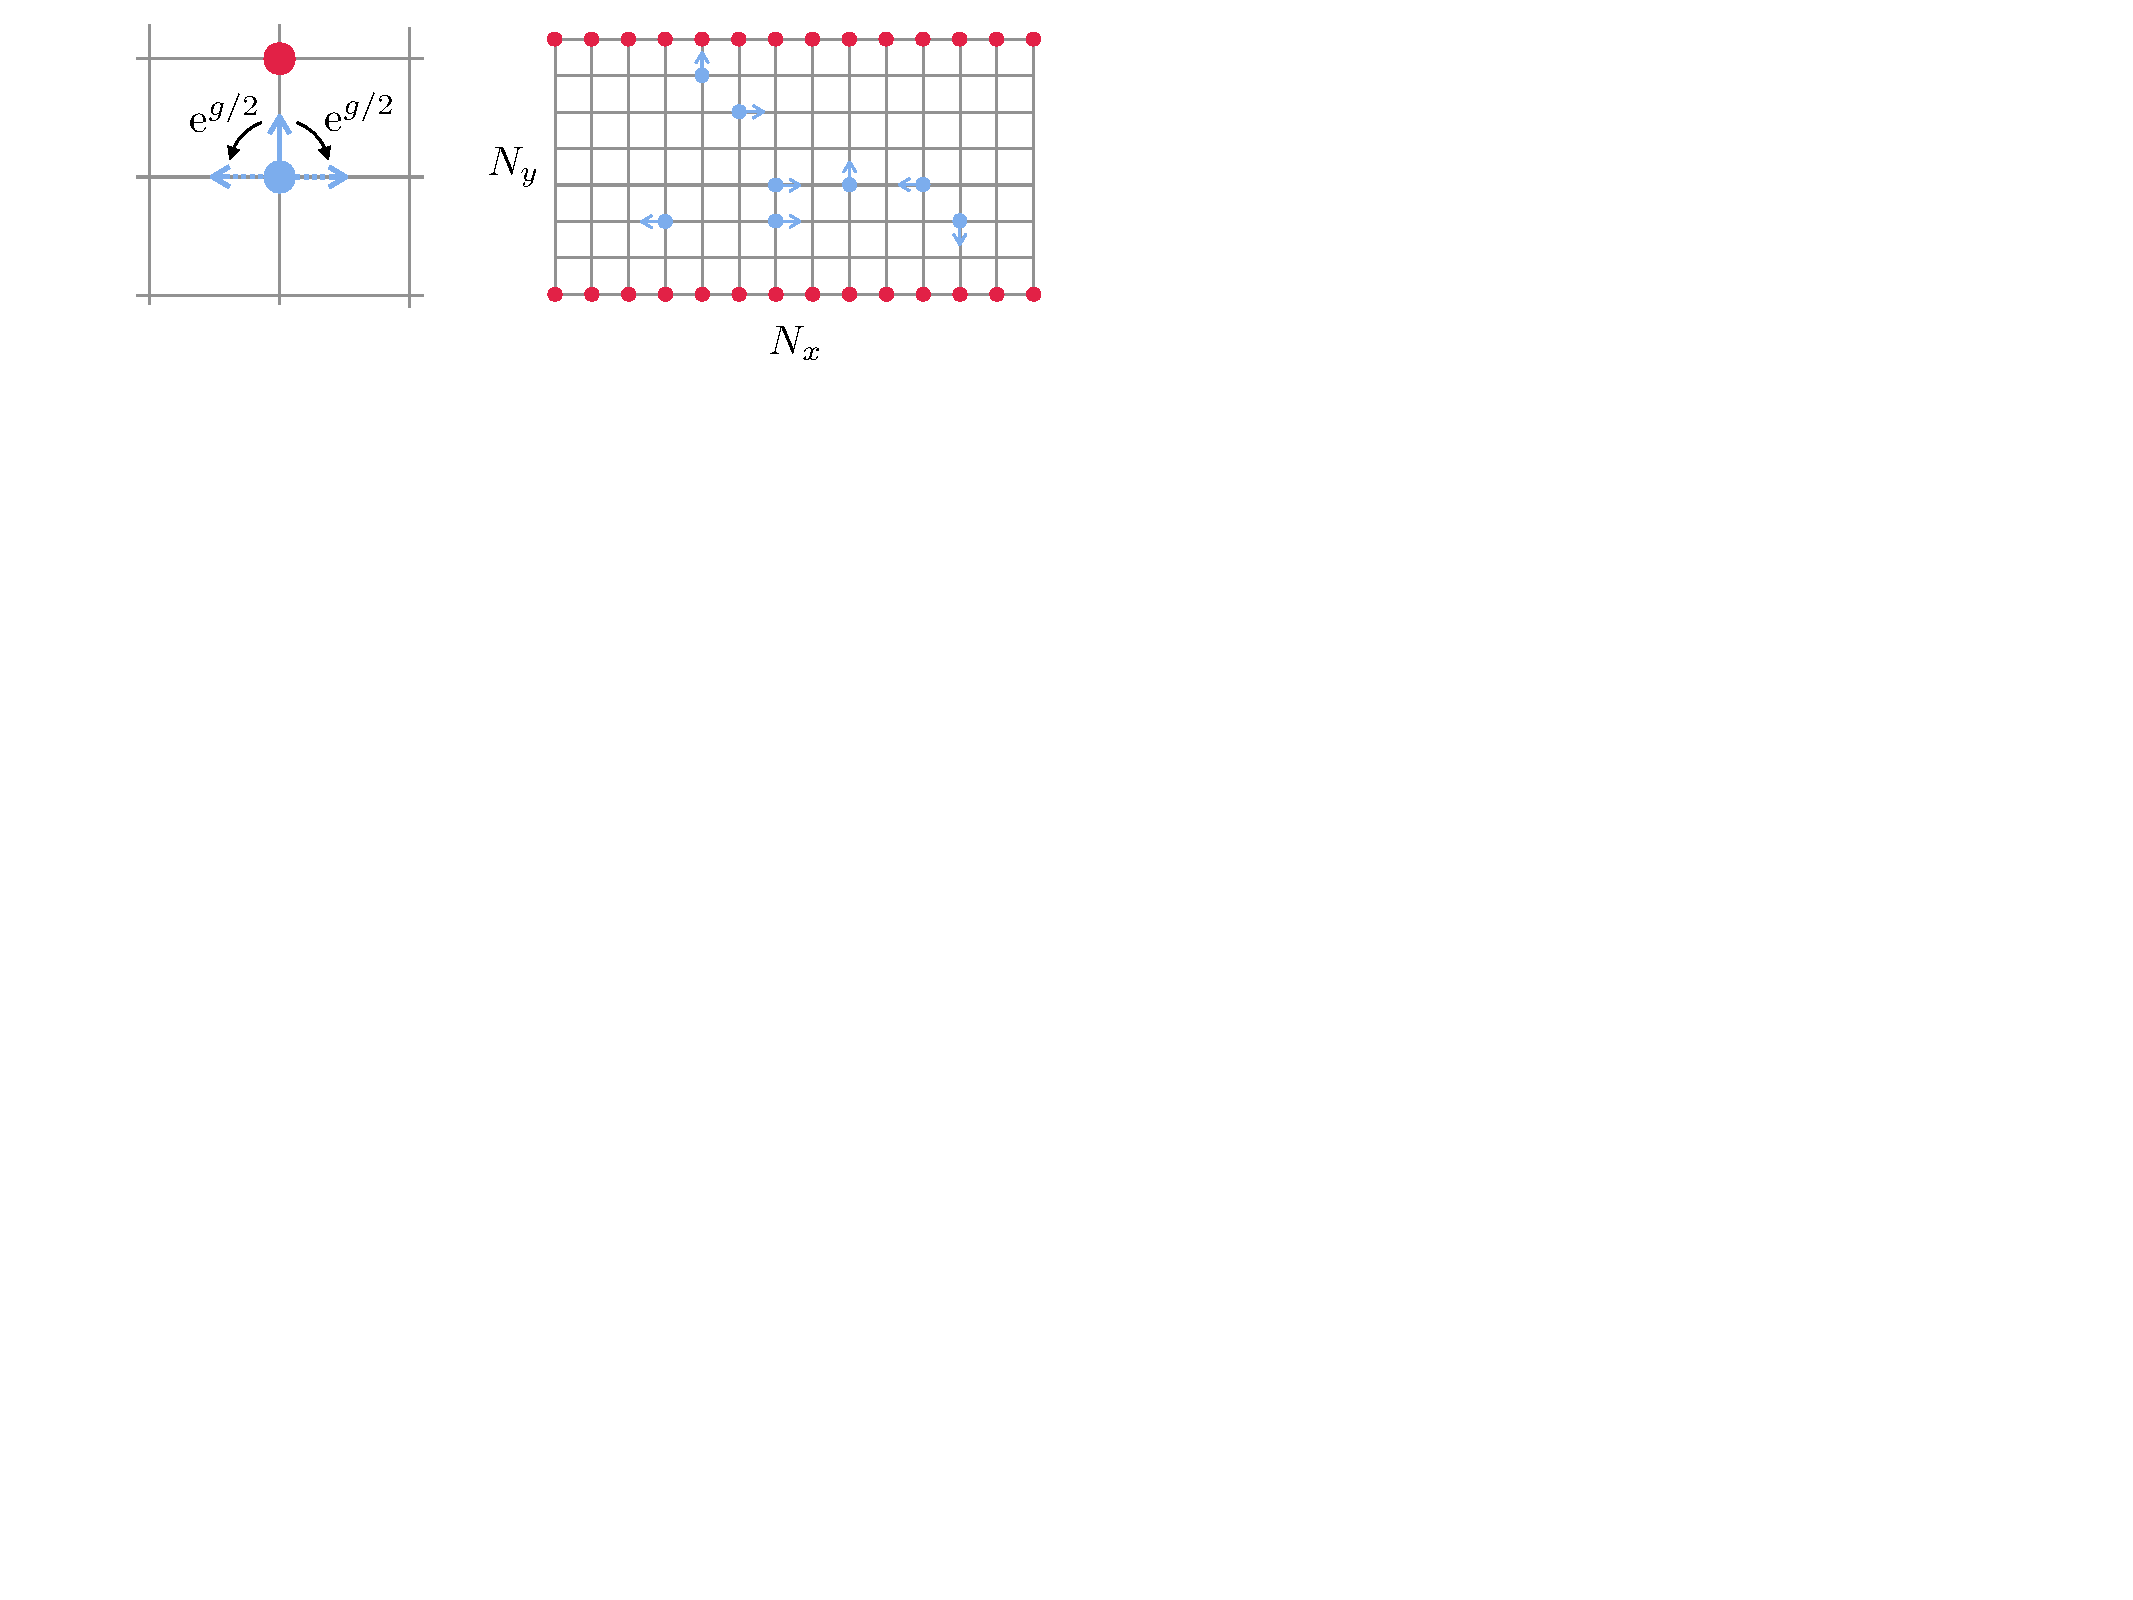
\includegraphics[width=.8\columnwidth]{sketch_lattice_channel.pdf}
    \caption{\label{fig:sketch_lattice_channel}Left: illustration of the reorientation induced by an obstacle (red dot) on a particle (blue dot) that faces it. Right: Periodic channel of size $N_x\times N_y$ with two walls of obstacles (top and bottom rows of red dots).}
\end{figure}

We consider a channel geometry where the top and bottom layers (at $y=-h$ and $y=h$) are occupied by obstacles, defining walls (see Fig.~\ref{fig:sketch_lattice_channel}, right). We maintain periodic boundary conditions in the $x$ direction. The dynamics of interacting active particles and swarms in such a configuration have been studied in the continuous case~\cite{armbruster2017swarming} and for a hybrid lattice method~\cite{kuhn2021lattice}. Note that these studies considered reflective boundary conditions, which slightly differ from our preferential alignment.

A fluid flow is imposed in the channel. For that, we assume that, in addition to their swimming motion and interactions, the active particles systematically experience a translational motion towards $x>0$. This is implemented as additional migration events to the next right \CC{site} with a rate $U_j = v_1[1-(2\,j/(N_y-1)-1)^2]$ that depends on their ordinate \CC{$j \in [0,N_y-1]$}, and thus on their distance to the boundary. We are here implicitly assuming that the channel has a width $2h$ and that the wall-normal coordinate is discretized as $y = h(2j/(N_y-1)-1)\in[-h,h]$. Such a profile mimics that of a Poiseuille flow describing the creeping motion of a viscous fluid in the channel, with no-slip boundary conditions at the walls. The fluid flow has gradients that also affect particle orientation. These effects are taken into account through an additional reorientation rate $\Omega_j = 2v_1 |y/h| = 2v_1|2j/(N_y-1)-1|$ \CC{CC: I think this expression is wrong (see comment below)} at which the particle will turn clockwise or anticlockwise depending on whether it is in the upper or lower half of the channel. \obs{The factor 2 is in the code but we should check if this makes sense.} 
\CC{CC: These effects are taken into account through an additional reorientation rate $\Omega_j = v_1 |y/h^2| = 2v_1|2j/(N_y-1)-1|/N_y$. (This is from where the factor 2 comes from. In the code we defined y as y/h, then we have an extra h in the denominator of $\Omega_j$ and in the code is equivalent to multiple for 2/Ny).}

\CC{maybe here it is also good if we prepare an image that schematize how the flow influences the particle.}

We choose the units of length so that the channel width is $h=1$ and time units so that the random reorientation rate is $\mu = 1$. Table~\ref{tab:parameters} summarizes the parameters of our model that remain after this choice, with some comments on those which we choose to fix and those to vary.
\begin{table}[h]
    \caption{\label{tab:parameters}Model parameters.}
    \begin{ruledtabular}
        \begin{tabular}{p{1.6cm}cp{4.2cm}}
            Resolution & $N_y$ & fixed to $25$, but larger values should be tested \\ \hline
            Box shape & $\lambda = N_x/N_y$ & fixed to $2$, but some larger values should be tested\\ \hline
            Density & $\rho = N_{\rm p} / (N_x\,N_y)$ & fixed to $0.3$, as a reasonable intermediate between ``too dilute'' and ``too packed''\\ \hline
            Alignment sensitivity & $g$ & weight of interactions w.r.t.\ noise; variations are crucial to exploring swarming behaviors\\ \hline
            Migration rate & $v_0$ & fixed to $100$, i.e., much faster than noise, but comparable to alignment for $g=\mathcal{O}(1)$\\ \hline
            Flow rate & $v_1$ & $v_1/v_0$ is an important parameter that we chose to vary
        \end{tabular}
    \end{ruledtabular}
\end{table}

\noindent\begin{tabular}{|p{\columnwidth}|}
\hline \textbf{The story we want to tell:} There are different regimes in parameter space where particles cluster at the boundaries, hindering their displacement in the channel. Can we use a global control of such swarms that will avoid clustering and enhance transport? \\ \hline
\end{tabular}

\section{Swarm statistics with no control}

\subsection{Order parameters and statistics}
Our objective here is to fix $N_y$, $\lambda$, $\rho$, and $v_0$ as in Tab.~\ref{tab:parameters} to explore the parameter plane $(g,v_1)$. To characterize different phases, we measure the classical order parameter given by the instantaneous mean particle orientation:
\begin{equation}
\Pi = |\boldsymbol{\Pi}|, \quad\mbox{with } \boldsymbol{\Pi}(t) = \frac{1}{N_{\rm p}}\sum_{k=1}^{N_{\rm p}} \boldsymbol{p}_{k}(t).
\label{eq:defPhia}
\end{equation}
The parameter $\Pi$  is close to 0 when the active particles are randomly oriented (\CC{CC: and if N particles form a band and other N particles another band in the opposite direction}), and close to 1 when they are all aligned in the same direction and form swarms. In the anisotropic channel geometry, it might also be interesting to monitor the orientation of the mean orientation vector $\boldsymbol{\Pi}$. In addition, we can use the clustering order parameter
\begin{equation}
\Psi(t) = \frac{1}{4N_{\rm p}}\sum_{k=1}^{N_{\rm p}} \# {\rm Neigh}(k),
\end{equation}
which is close to 0 if particles are dilute and isolated, and close to 1 if they form dense clusters.

Because of our non-homogeneous settings, it is interesting to introduce statistics as a function of the distance to the boundary. A natural quantity to introduce is the wall-normal mass profile
\begin{equation}
N_j(t) = \sum_{\CC{k} = 1}^{N_{\rm p}} \delta_{Y_{\CC{k}},j} = \sum_i M_{i,j},
\end{equation}
where $N$\CC{($M$ ?)} denotes the mass matrix whose element $(i,j)$ is 0 or 1, depending whether lattice site $(i,j)$ is empty or contains a particle. Using these weights, we can define the average distance to the boundary
\begin{equation}
  \Delta(t) = \sum_j \frac{N_j(t)}{N_{\rm p}} \min(j,N_y-j).
\end{equation}
This quantity can be useful to characterize whether the particles are concentrated in the center of the channel or at a wall.  Additionally, we can extend the order parameters to account for a vertical dependence. For the orientation, one introduces
\begin{equation}
  \boldsymbol{\Pi}_j = \frac{1}{N_j} \sum_{k=1}^{N_{\rm p}} \boldsymbol{p}_{k}\,\delta_{Y_{k},j}
\end{equation}
with the convention that $\boldsymbol{\Pi}_j(t) = 0$ if $N_j(t)=0$. For the clustering order parameter, one similarly writes
\begin{equation}
  \Psi_j =  \frac{1}{4N_j}\sum_{\CC{k}=1}^{N_{\rm p}} \# {\rm Neigh}(\CC{k})\,\delta_{Y_{\CC{k}},j},
\end{equation}
with again the same convention as for $\boldsymbol{\Pi}$ (set to zero when $N_j=0$). The relations with global order parameters are
\begin{equation}
  \boldsymbol{\Pi} = \sum_j \frac{N_j}{N_{\rm p}}\,\boldsymbol{\Pi}_j \quad\text{and}\quad \Psi = \sum_j \frac{N_j}{N_{\rm p}}\,\Psi_j.
\end{equation}
There is a question that arose during our discussions regarding the way one accounts for $y$ dependence in estimating global orders. In particular, there is another way to extract information on swarm order from $\boldsymbol{\Pi}_j$, which consists in computing their moduli before summing over $j$. This could lead to different results when, for instance, the particles form several bands with opposite velocities.

A last comment concerns averages. We are of course willing to do statistical measurements on all these observables. In our settings, we expect that each configuration, with or without control, will reach after a long-enough time, an ergodic, statistically  stationary state. In this regime, physically relevant statistics should be given by the time average. In principle, we should thus do time average. However, it seems that doing rather an average over iterations does not make a big difference. This is illustrated on Fig.~\ref{fig:compare_times}. It seems there that physical time runs slightly slower during transients, both at beginning of the simulation and around $t=100$ when a transition occurs. This comes from the fact that in the steady configuration, which consists of bands, global rotation and migration rates are longer than in a situation where more particles can rotate or move. In the sequel, we are considering averages over events only, but this point should be kept in mind. \obs{There is a point which is still unclear to me on how to define time, related to the fact that we removed the ``null events'' (when nothing changes in the configuration).} 
\begin{figure}[h!]
   \centering
   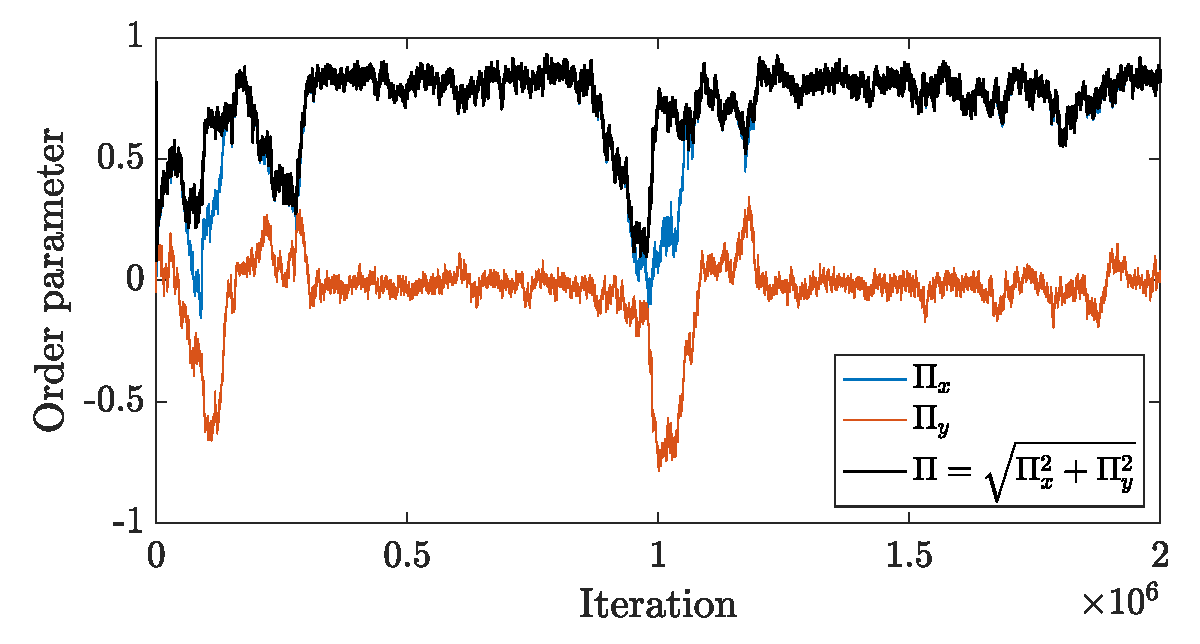
\includegraphics[width=.38\textwidth]{ord_param_phi_g1.75_v1_15_fn_iter}\\
   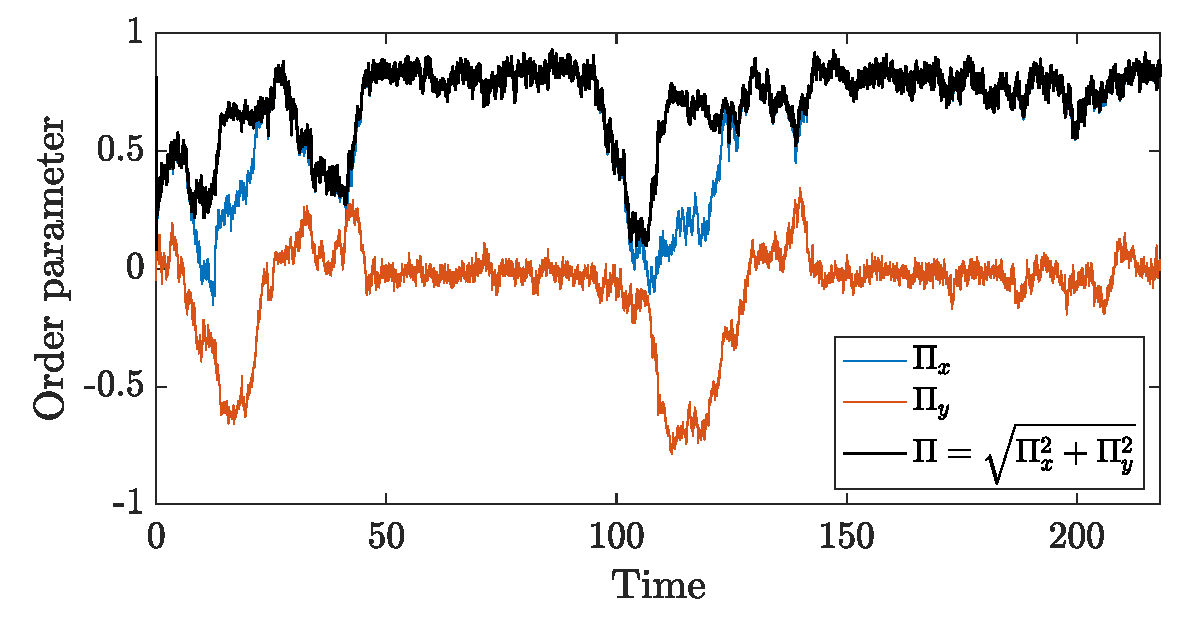
\includegraphics[width=.38\textwidth]{ord_param_phi_g1.75_v1_15_fn_time}
   \vspace{-10pt}
   \caption{\label{fig:compare_times} Order parameters $\Pi$ for $g=1.75$ for $v_1=15$ as a function of iteration (up) and of physical time (down).}
\end{figure}

We next proceed to characterizing swarm statistical properties, beginning with the absence of external flow.

\begin{figure*}[t!]
   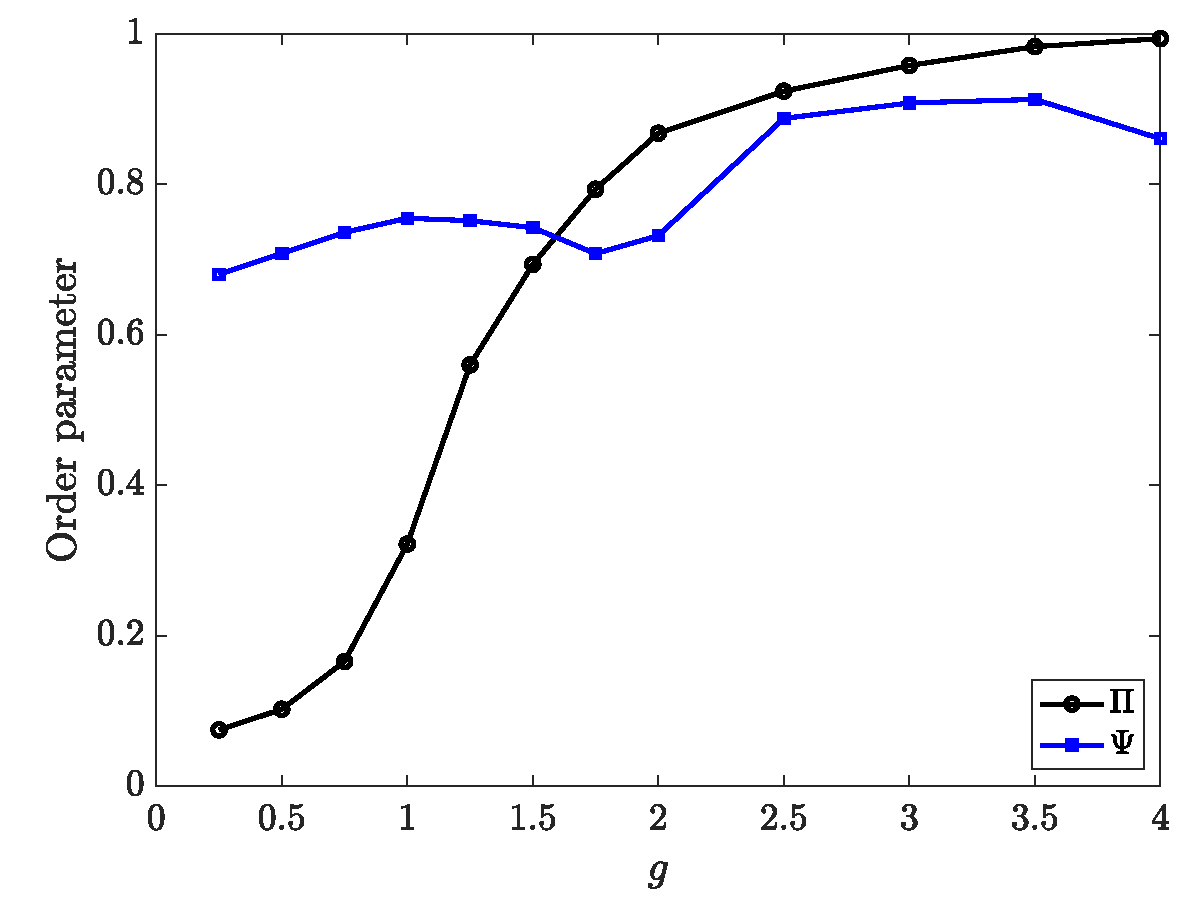
\includegraphics[width=.32\textwidth]{ord_param_v1_15_fng}
   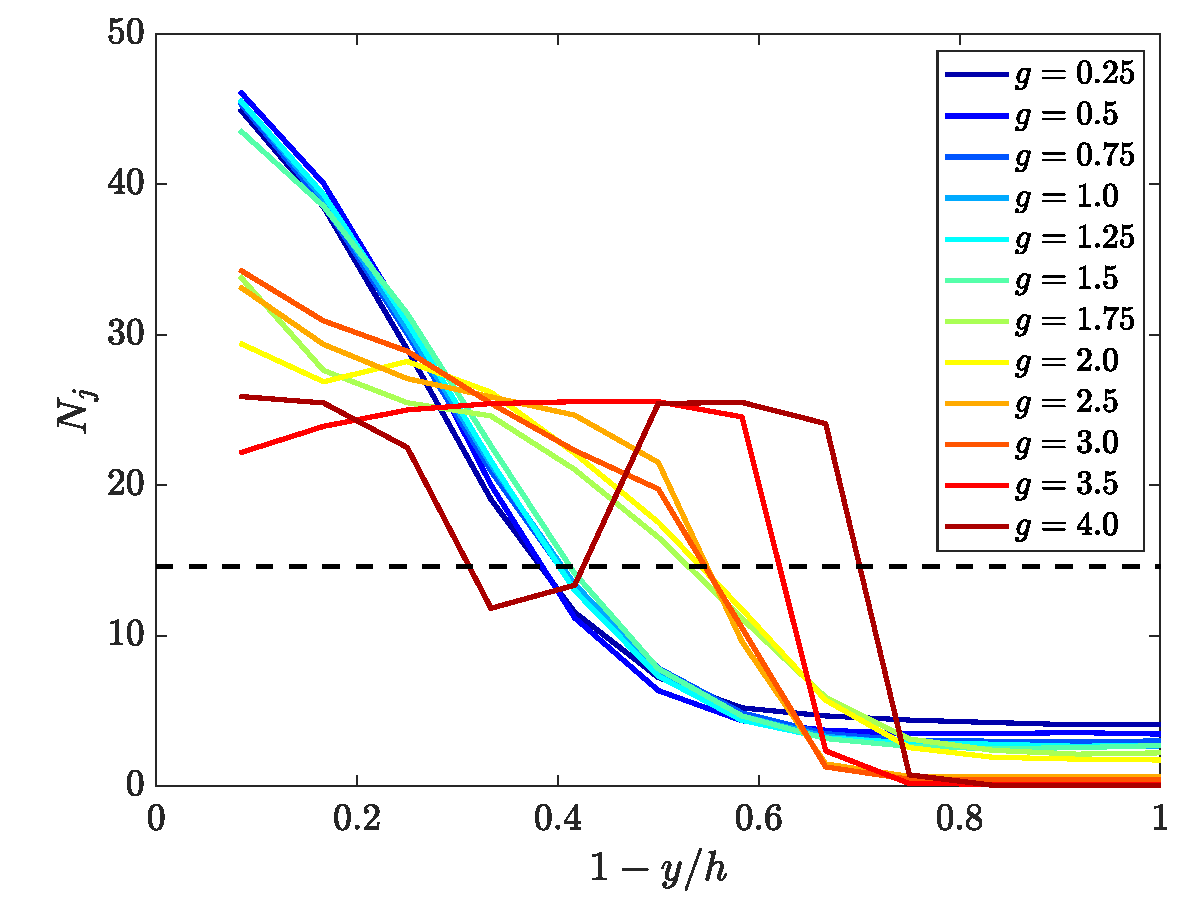
\includegraphics[width=.32\textwidth]{mean_density_v1_15_fny}
   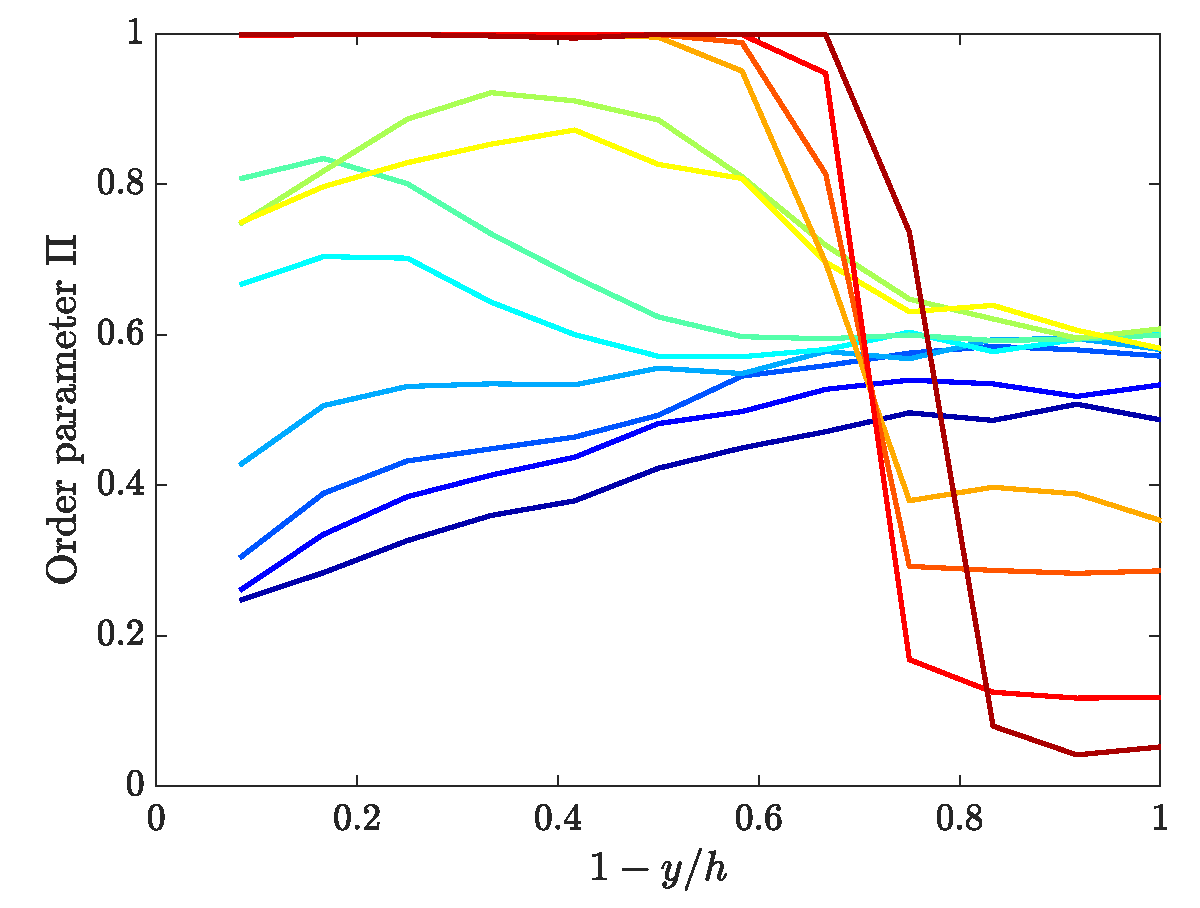
\includegraphics[width=.32\textwidth]{ord_param_phi_v1_15_fny}
   \caption{\label{fig:ordparam_noflow} Left: Order parameters $\Pi$ and $\Psi$ as a function of $g$ for $v_1=15$. Center: Mass profile $N_j$ as a function of the distance to the wall $1-y/h = 2j/(N_y-1)$; The dashed line shows a uniform distribution. Right: Order parameter \CC{$\Pi_j$} as a function of the distance to the wall. \CC{CC: x-axis of the center and right panels should go from 0 up to 2? or we can directly show y/h like in fig.5}}
   \vspace{10pt}
   \hspace{-10pt}
   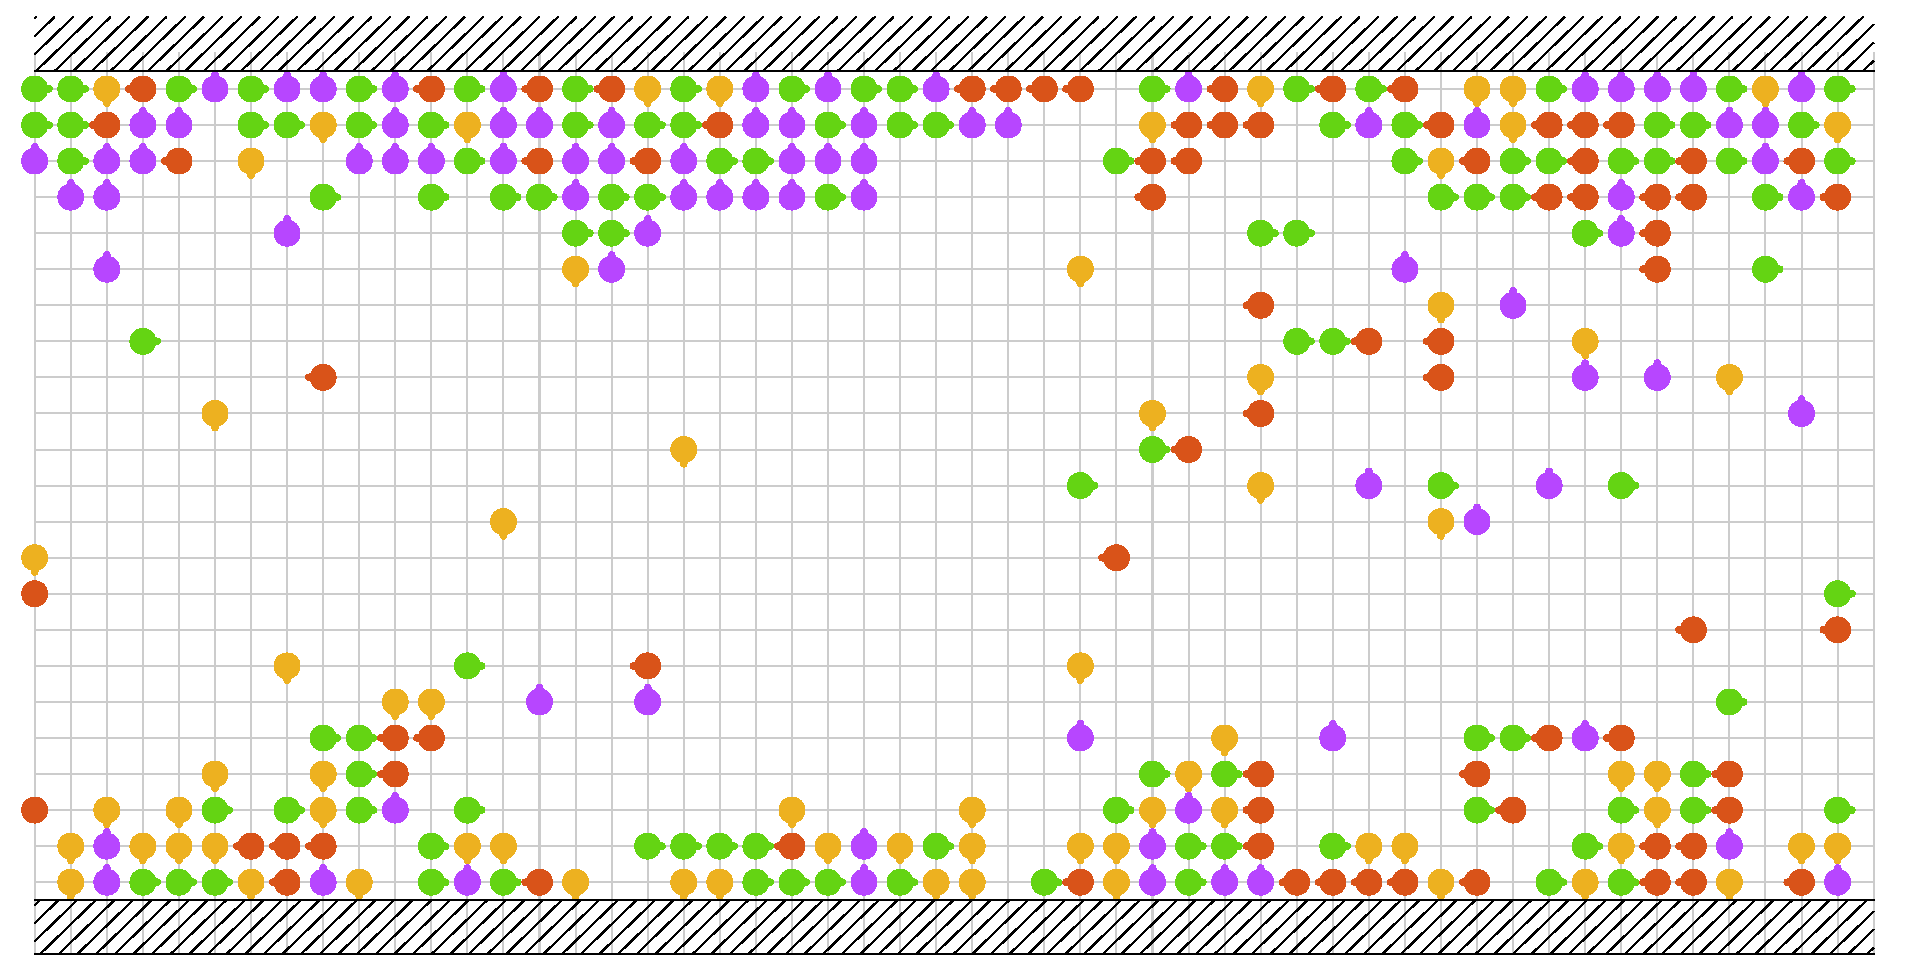
\includegraphics[width=.25\textwidth]{snap_g0.25_v1_15_t2e6}\!\!
   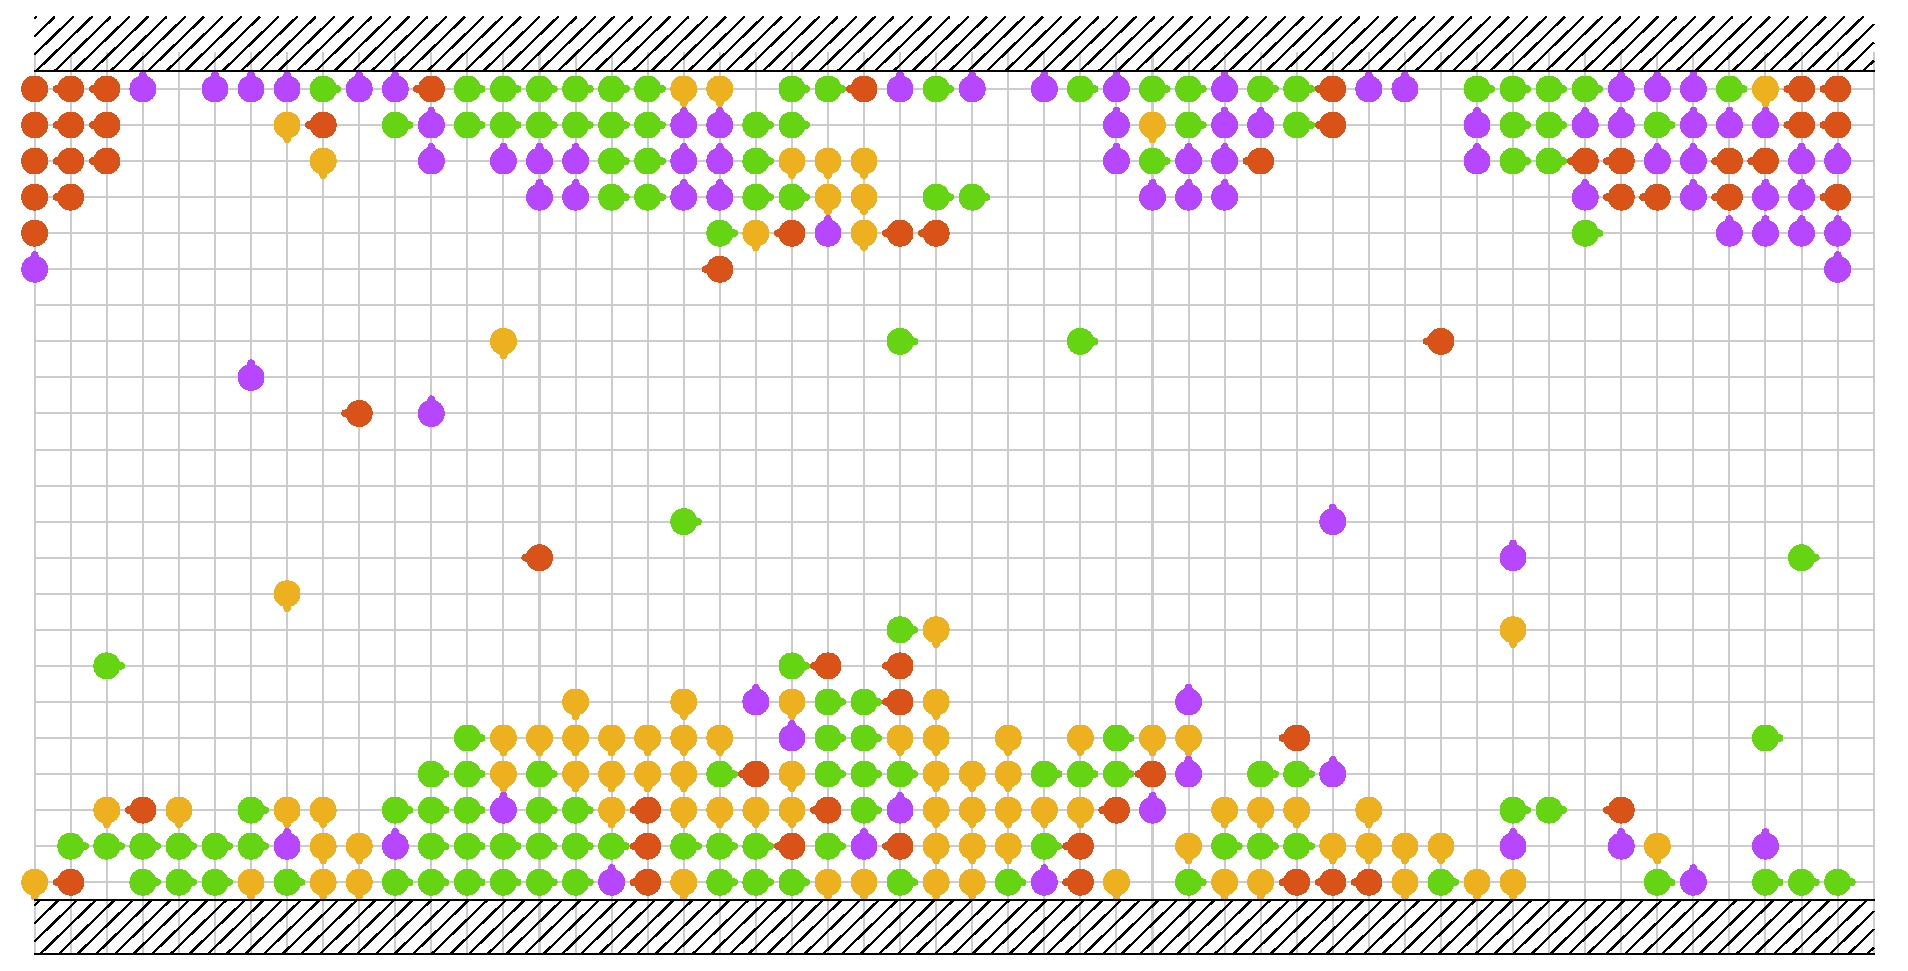
\includegraphics[width=.25\textwidth]{snap_g0.75_v1_15_t2e6}\!\!
   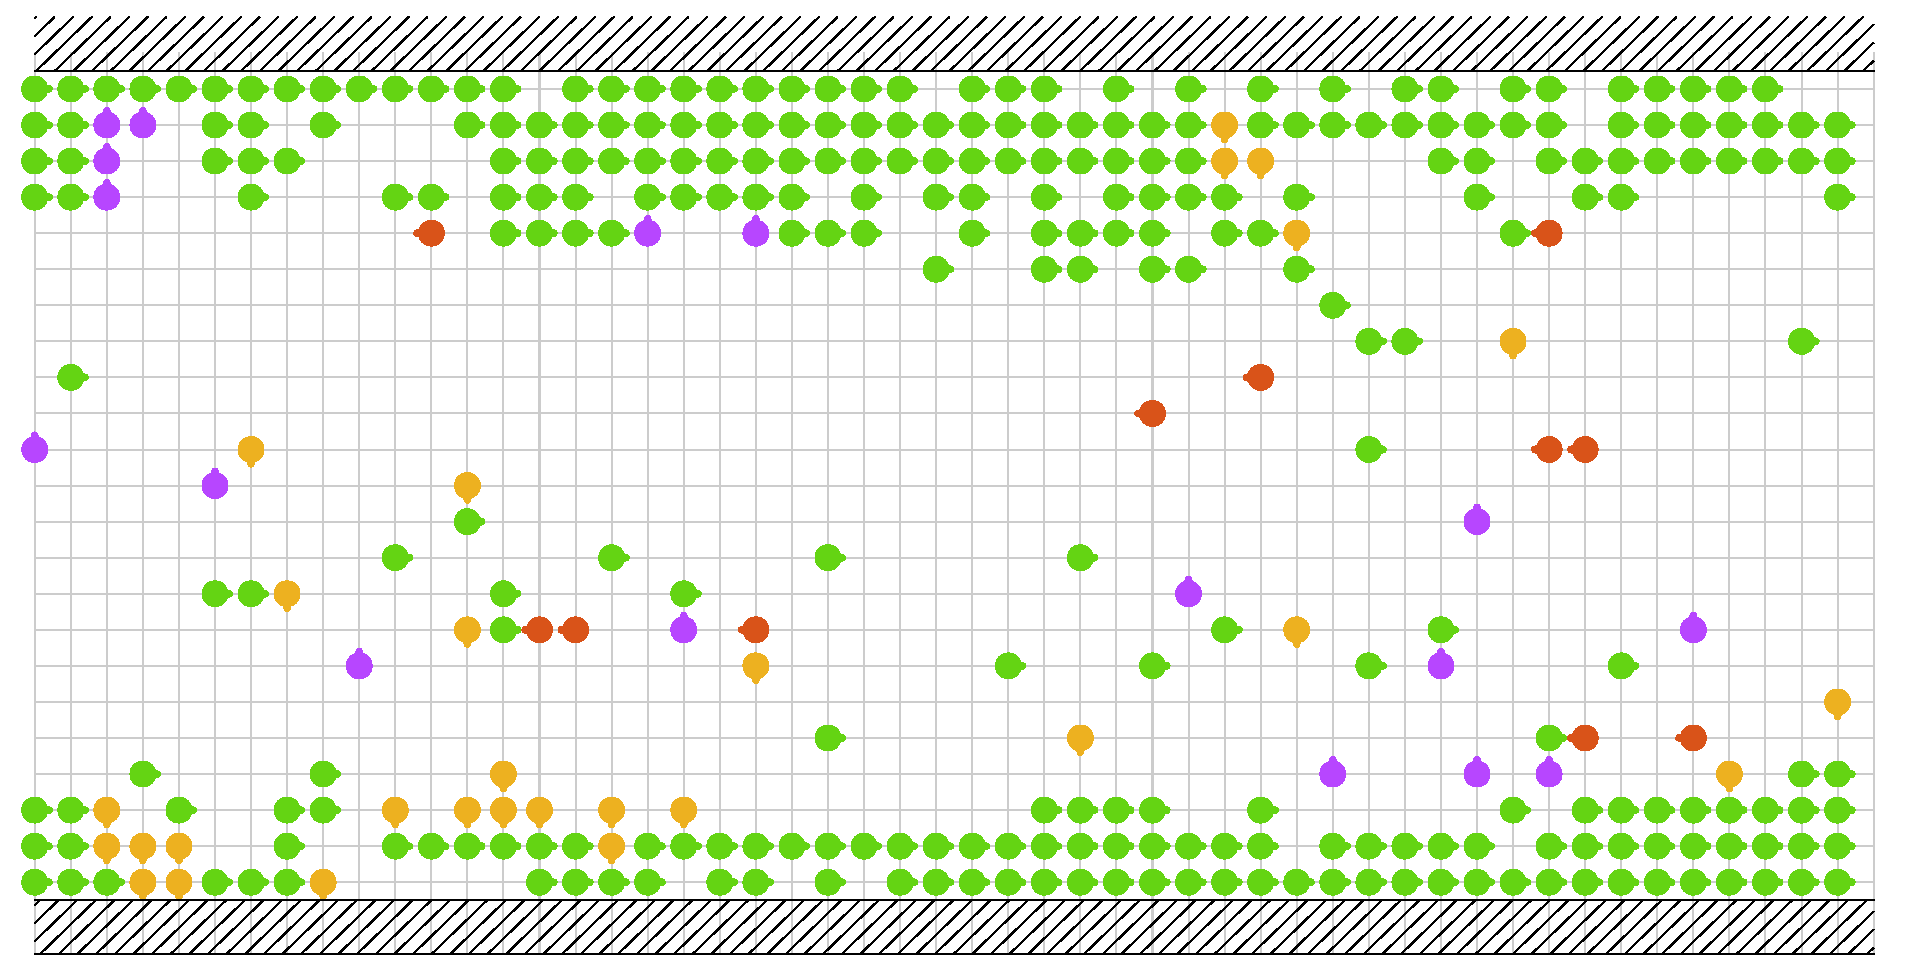
\includegraphics[width=.25\textwidth]{snap_g1.5_v1_15_t2e6}
   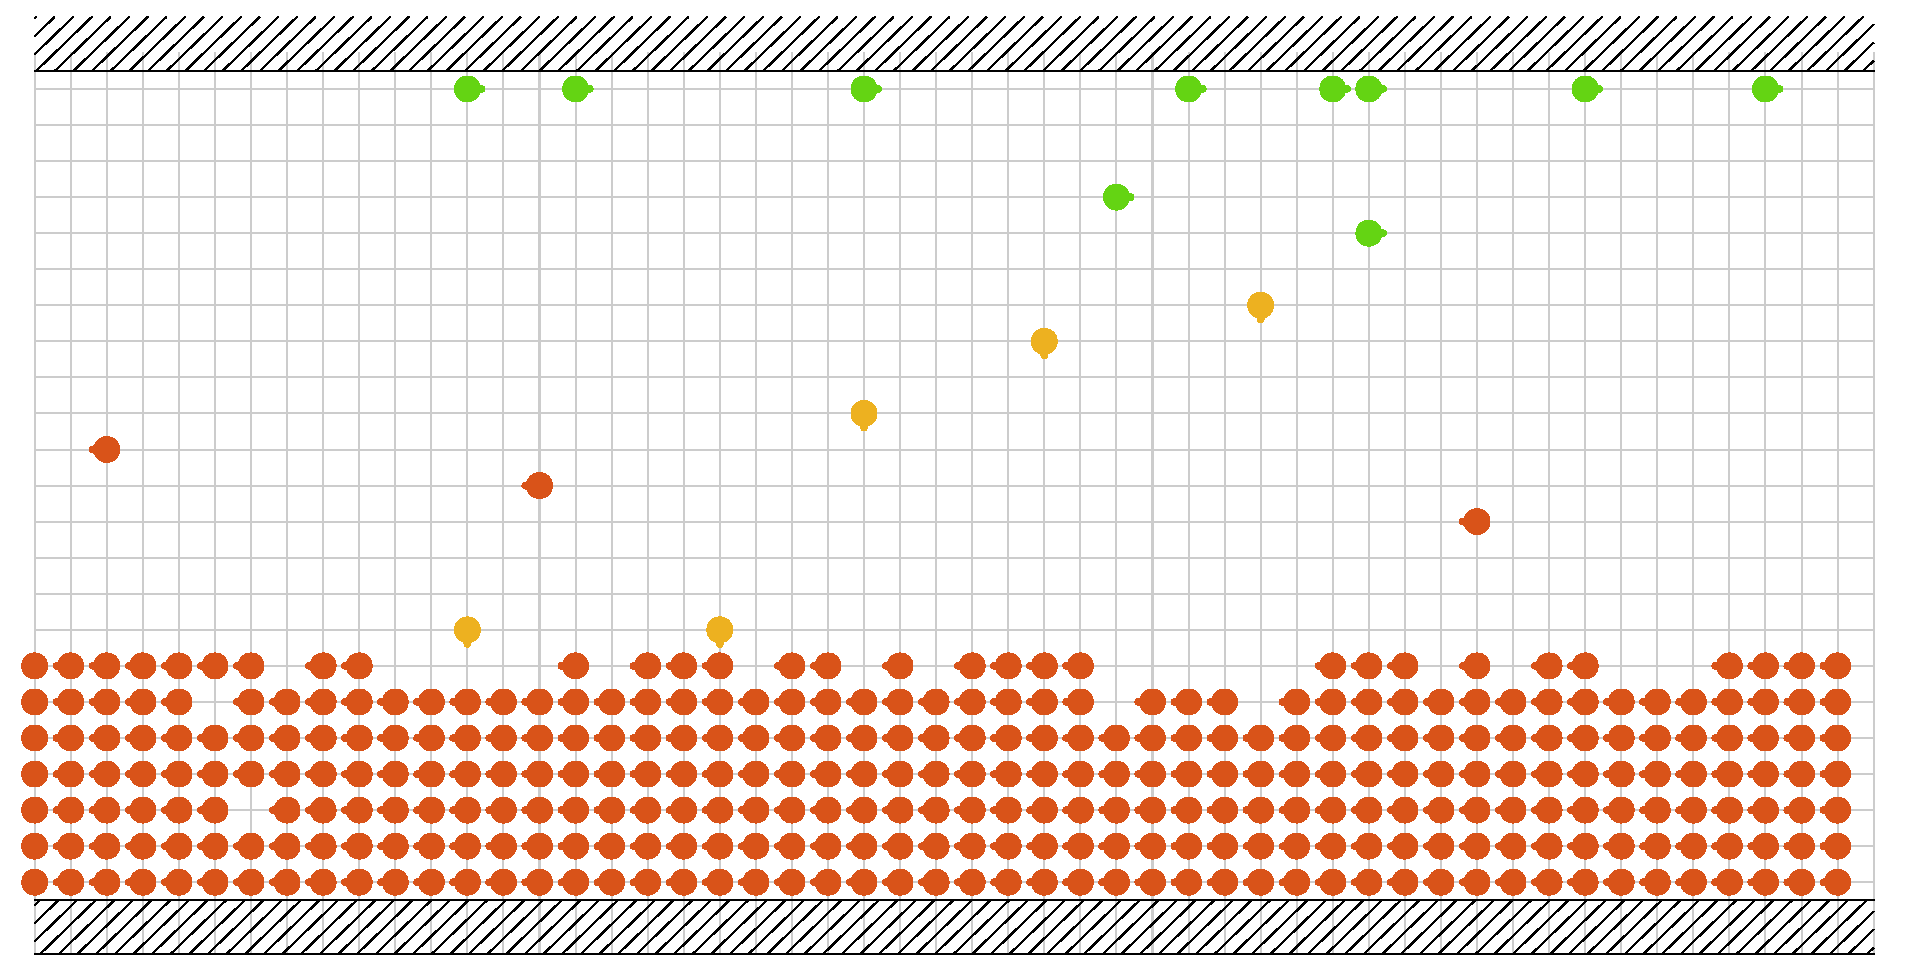
\includegraphics[width=.25\textwidth]{snap_g3_v1_15_t2e6}
   \caption{\label{fig:snapshots} Snapshots of the lattice configuration for $v_1=15$ and increasing $g$ (0.5, 0.75, 1.5, and 3 from left to right). Particles oriented to the right are shown in green, to the left in red, to the top in purple and to the bottom in yellow, respectively.}
\end{figure*}

\subsection{The case with no flow}
Measurements were conducted with $v_1=15$, while varying $g$, and the results are presented in Fig.~\ref{fig:ordparam_noflow}. \obs{(I didn't have the data for $v_1=0$, but I guess this should not change the qualitative gross behaviors.)} As anticipated, the left panel illustrates that the order increases with alignment. However, at small values of $g$, particles tend to form clusters at the boundaries. Consequently, $\Phi$ \CC{($\Pi_j$ ?)} exhibits larger values at small $g$'s than expected in the case of periodic boundary conditions. It is also noteworthy that the clustering order parameter, $\Psi$, is not particularly effective in distinguishing between the various possible phases, as it assumes relatively large values across all $g$ values. Nevertheless, we retain it in the analysis, considering that it might provide important information when implementing policies.

As an indication of clustering at the walls, the wall-normal mass profile $N_j$, depicted in the central panel, notably peaks near the boundary. This effect becomes more pronounced at the smallest values of $g$, even if, as seen from the right panel, the particles exhibit no order. For larger $g$ values, concentration aligns with order, and the active particles organize into bands where they are uniformly aligned. Illustrations of the various configurations that can be reached by the swarms are given in the lower panels of Fig.~\ref{fig:snapshots}. One observes, at small $g$'s, the formation of mountain-like clusters at the boundaries. At large values of $g$, the particles rather form bands that can occupy both boundaries or only one of the two.

\begin{figure}[h!]
   \begin{minipage}{.24\textwidth}
   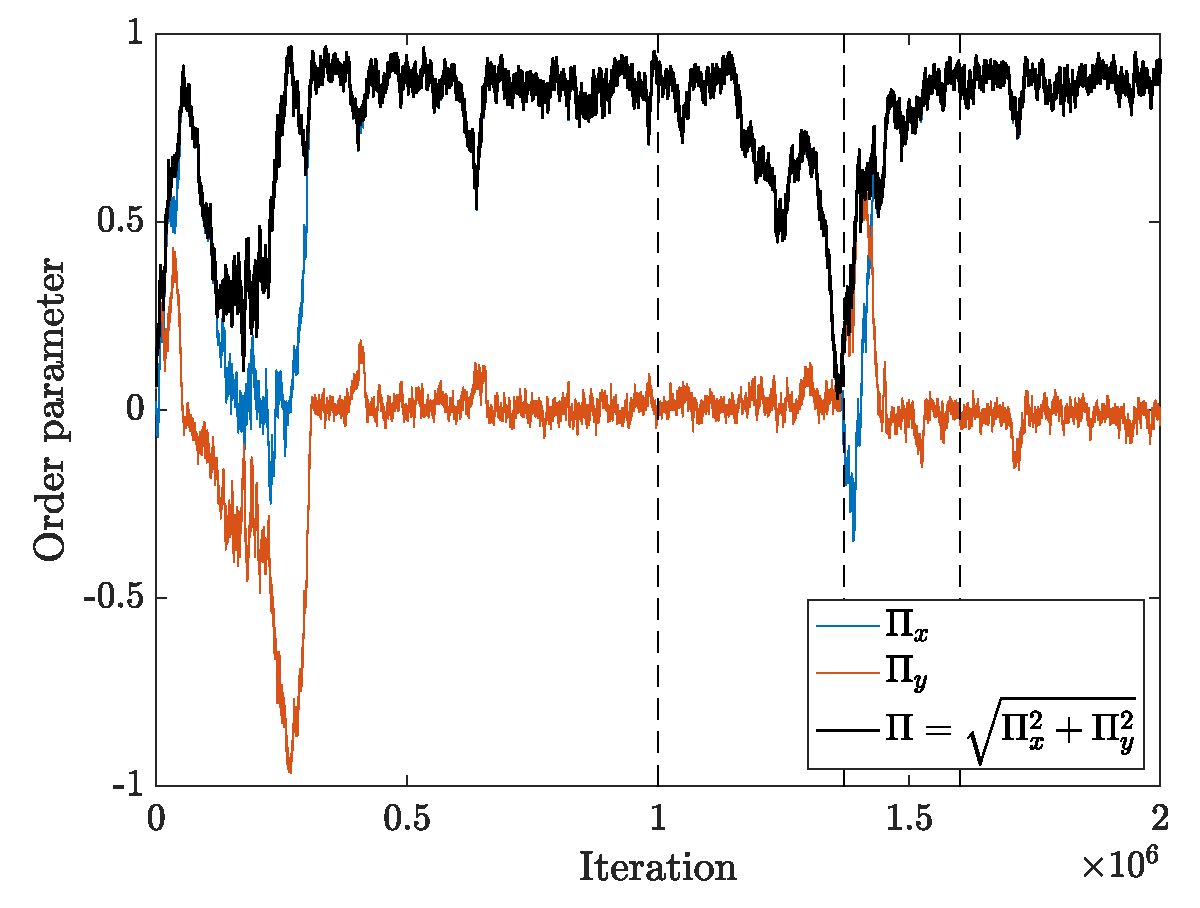
\includegraphics[width=\textwidth]{ord_param_phi_g2_v1_15}
   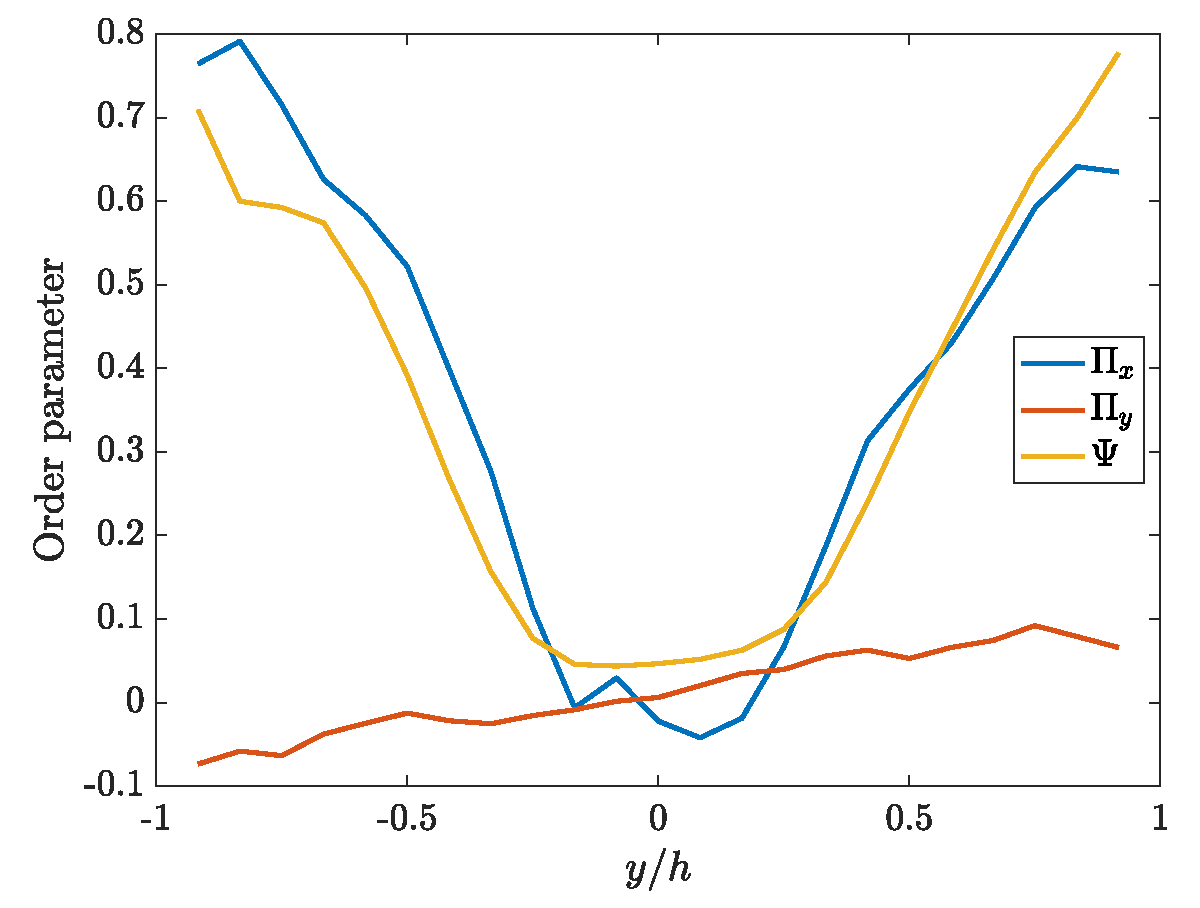
\includegraphics[width=\textwidth]{ord_param_phi_g2_v1_15_fny}
   \end{minipage}
   \hspace{-5pt}
   \begin{minipage}{.24\textwidth}
   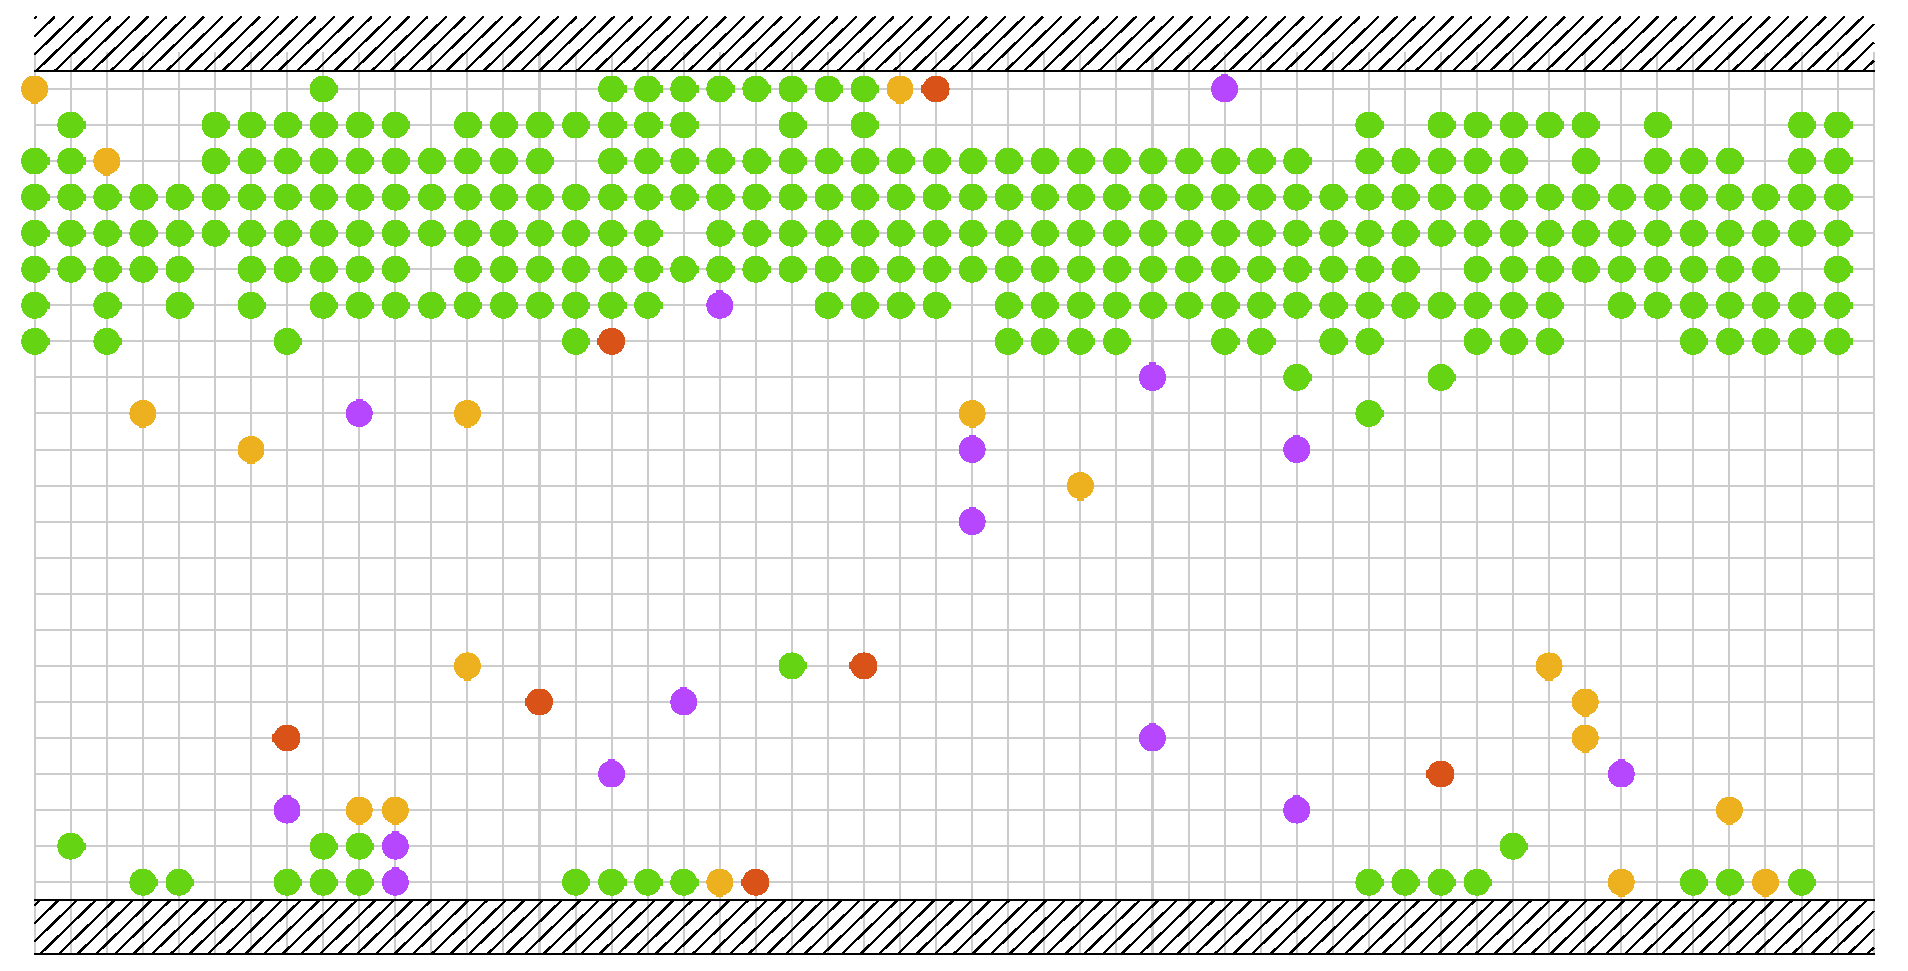
\includegraphics[width=\linewidth]{snap_g2_v1_15_t1e6}\\[4pt]
    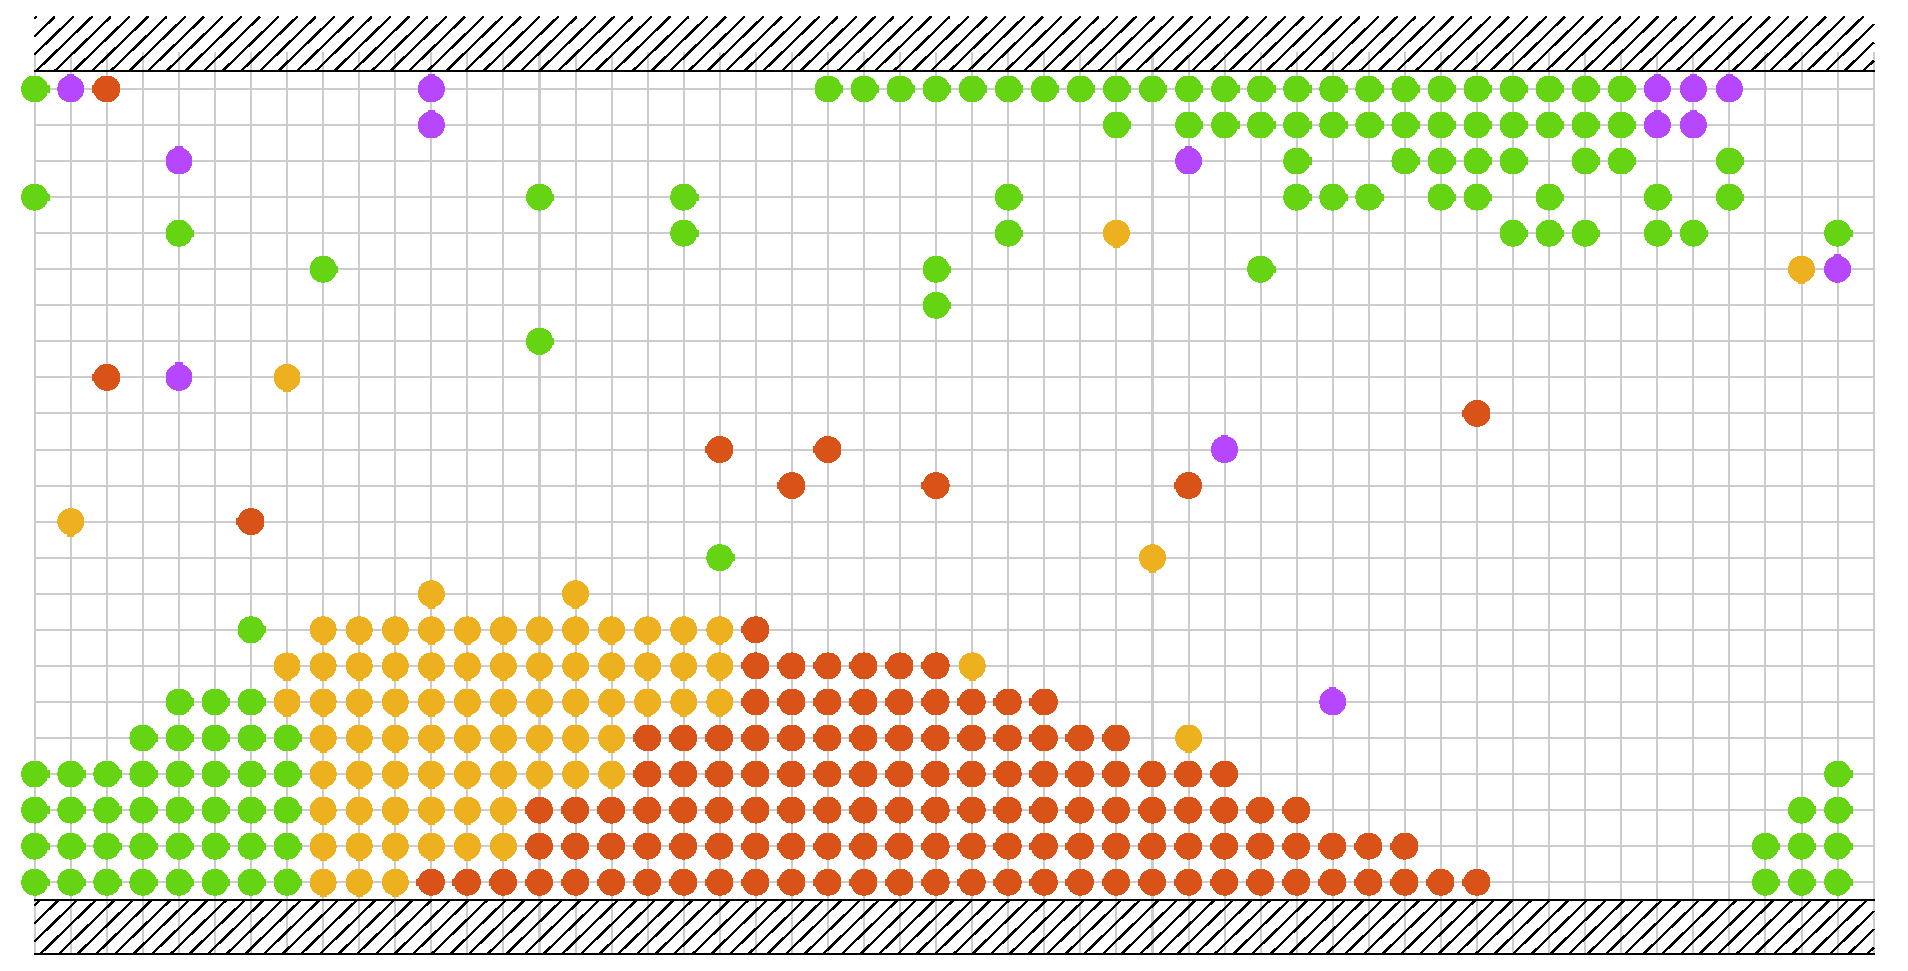
\includegraphics[width=\linewidth]{snap_g2_v1_15_t1.37e6}\\[4pt]
    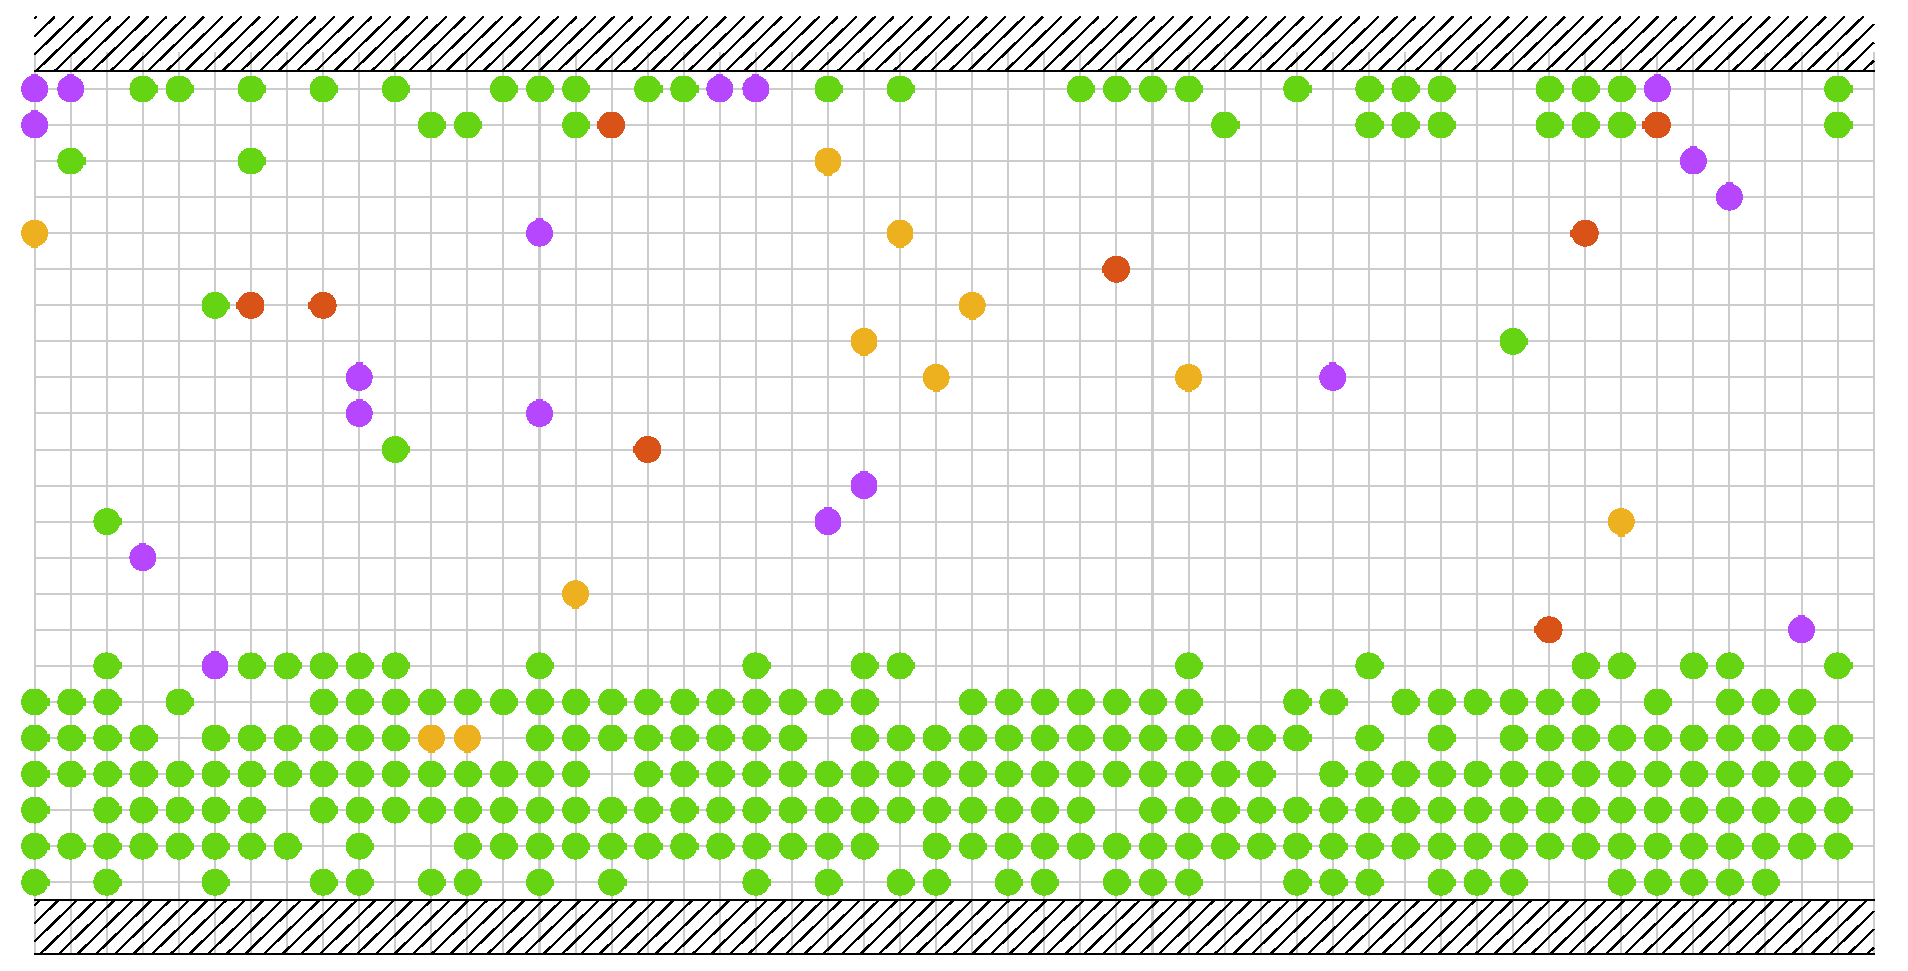
\includegraphics[width=\linewidth]{snap_g2_v1_15_t1.6e6}
    \end{minipage}
    \caption{\label{fig:g2_v1_15}Top, left: Time evolution of the orientation order parameters $\Pi$, $\Pi_x$ and $\Pi_y$ for $v_1=15$ and $g=2$. Bottom, left: $y$-dependent order parameter $\Pi_j$ averaged in time from iteration $4\times10^5$. Right panels: Configurations of the lattice at the three different times $t_1<t_2<t_3$ (from top to down), instants shown as vertical dashed lines in the top-left panel.}
\end{figure}
\begin{figure*}[t!]
   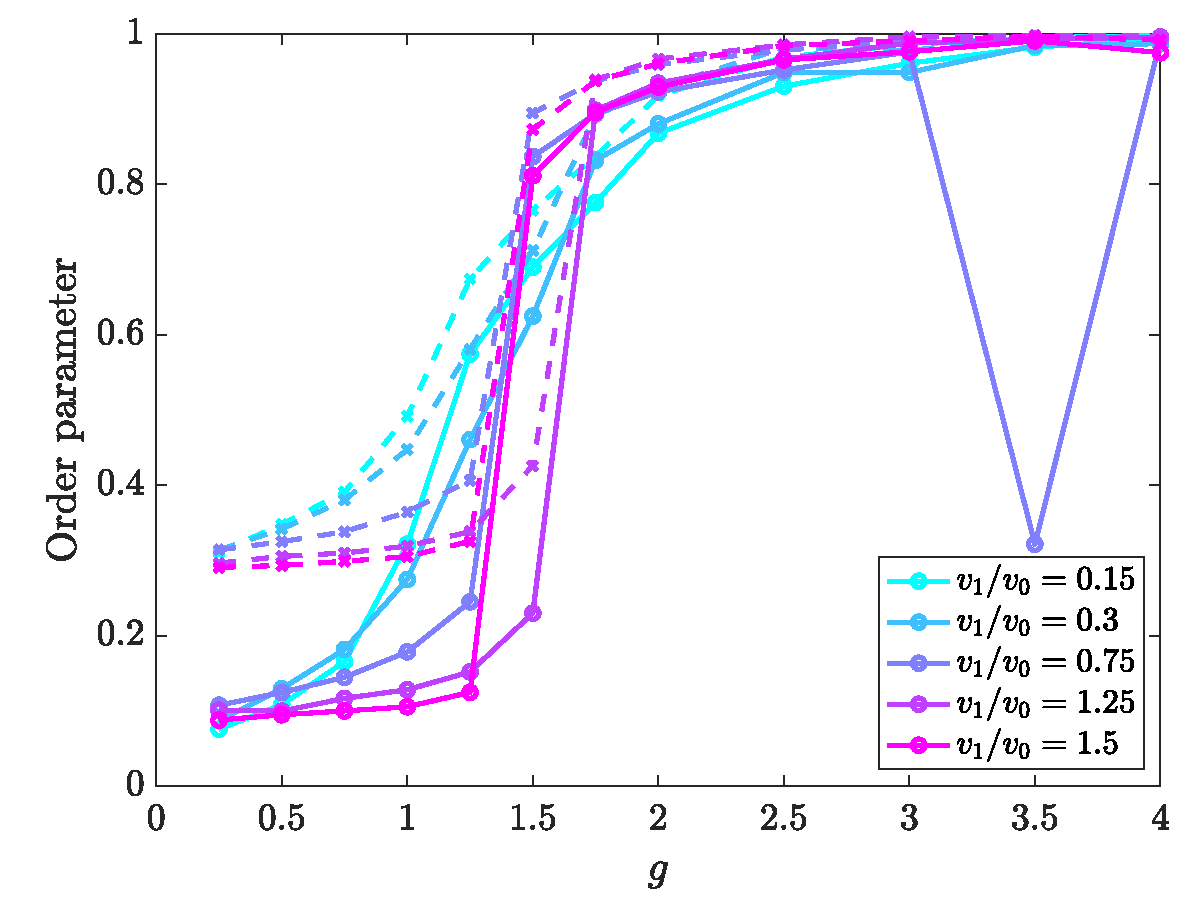
\includegraphics[width=.32\textwidth]{ord_param_var_v1_fng}
   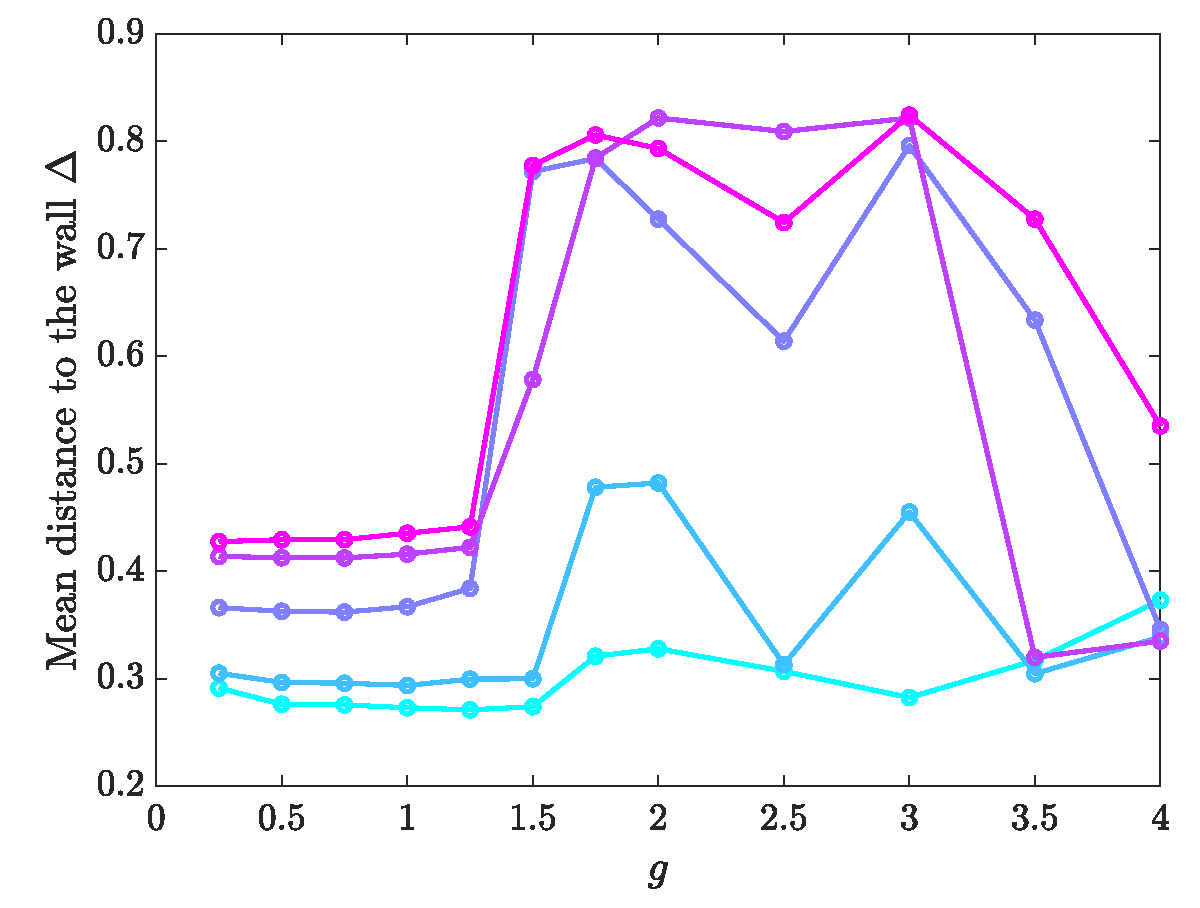
\includegraphics[width=.32\textwidth]{mean_dist_var_v1_fng}
   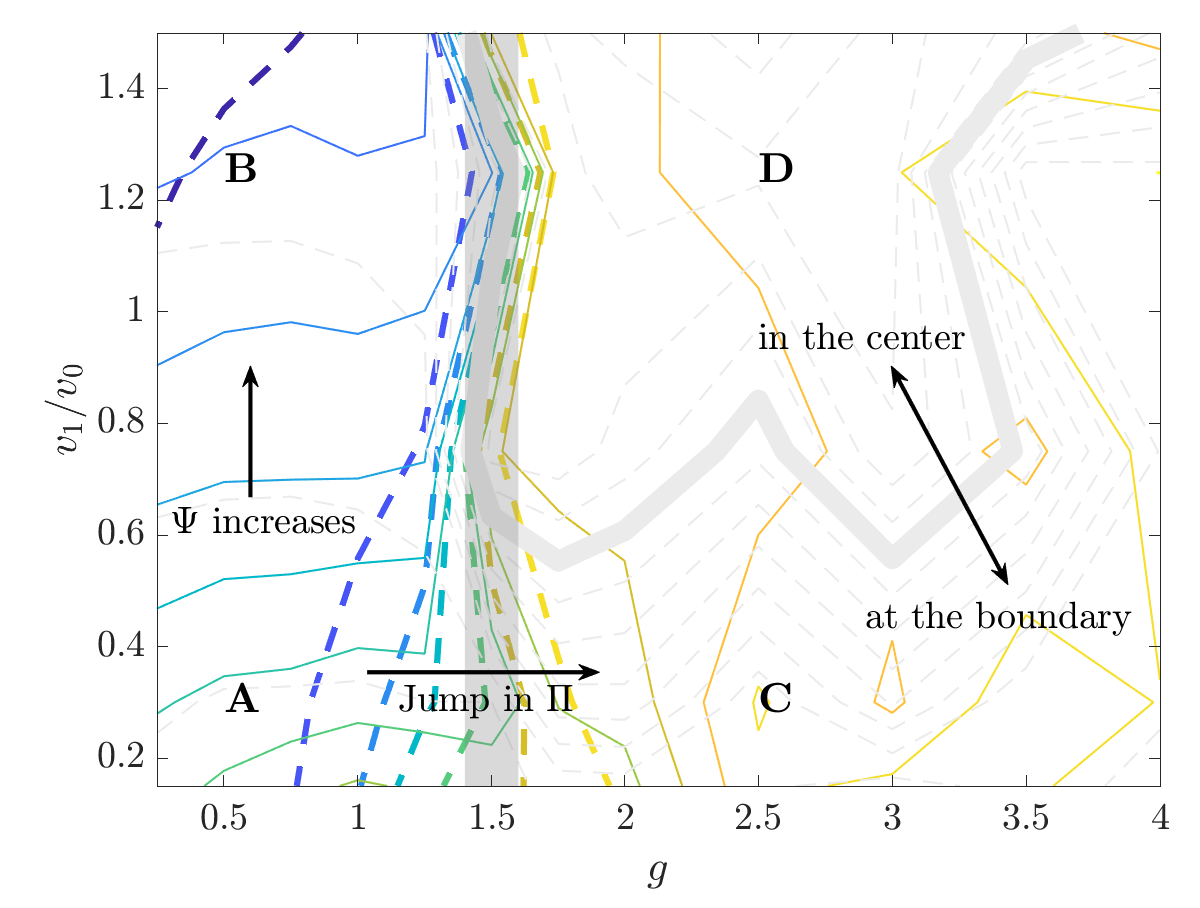
\includegraphics[width=.32\textwidth]{ord_param_fnv1_and_g}
   \caption{\label{fig:param_space} Left: Order parameters $\Pi$ as a function of $g$ for various $v_1$ (solid lines); The dashed lines uses the definition where the modulus is taken before the average w.r.t.\ $y$. Center: Average distance to the wall $\Delta$. Right: Phases in the $(g,v_1)$ parameter space. Bold dashed lines are the contour lines of $\Pi$, thin solid lines those of $\Psi$ and gray dashed lines those of $\Delta$.}
   \vspace{10pt}
   \hspace{-10pt}
   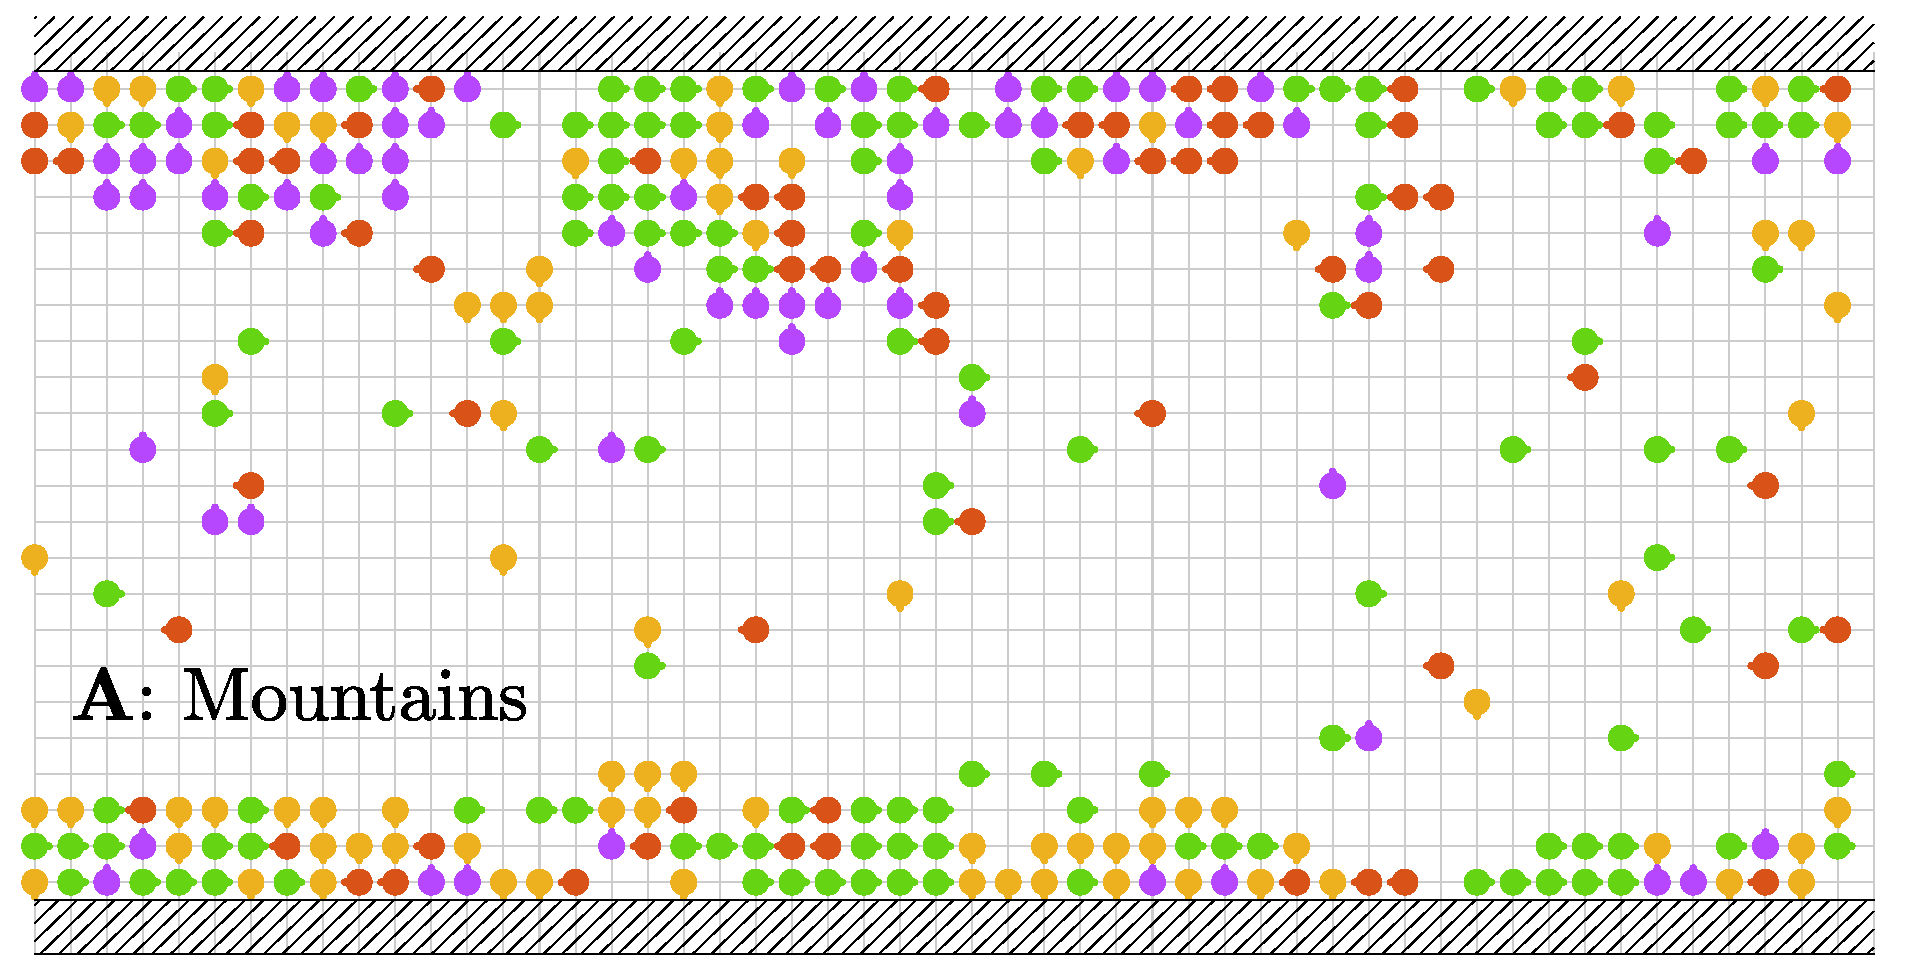
\includegraphics[width=.25\textwidth]{snap_g0.5_v1_30_t2e6}\!\!
   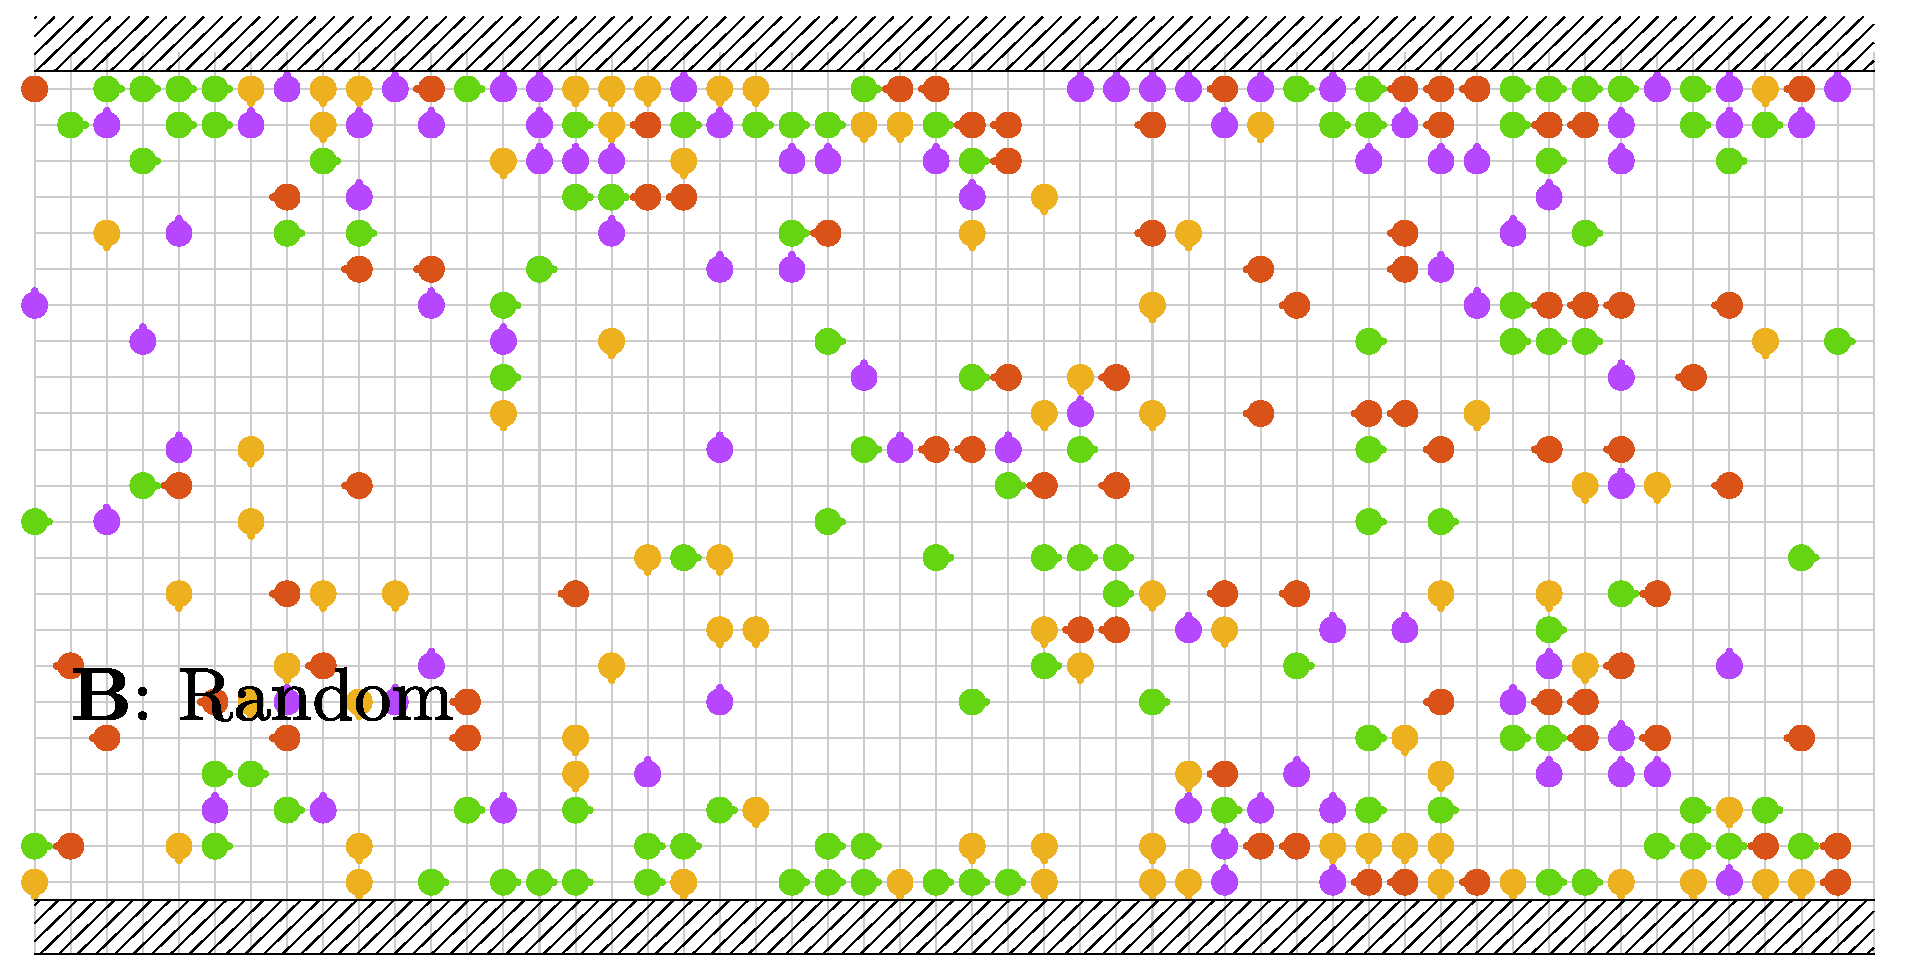
\includegraphics[width=.25\textwidth]{snap_g0.5_v1_125_t2e6}\!\!
   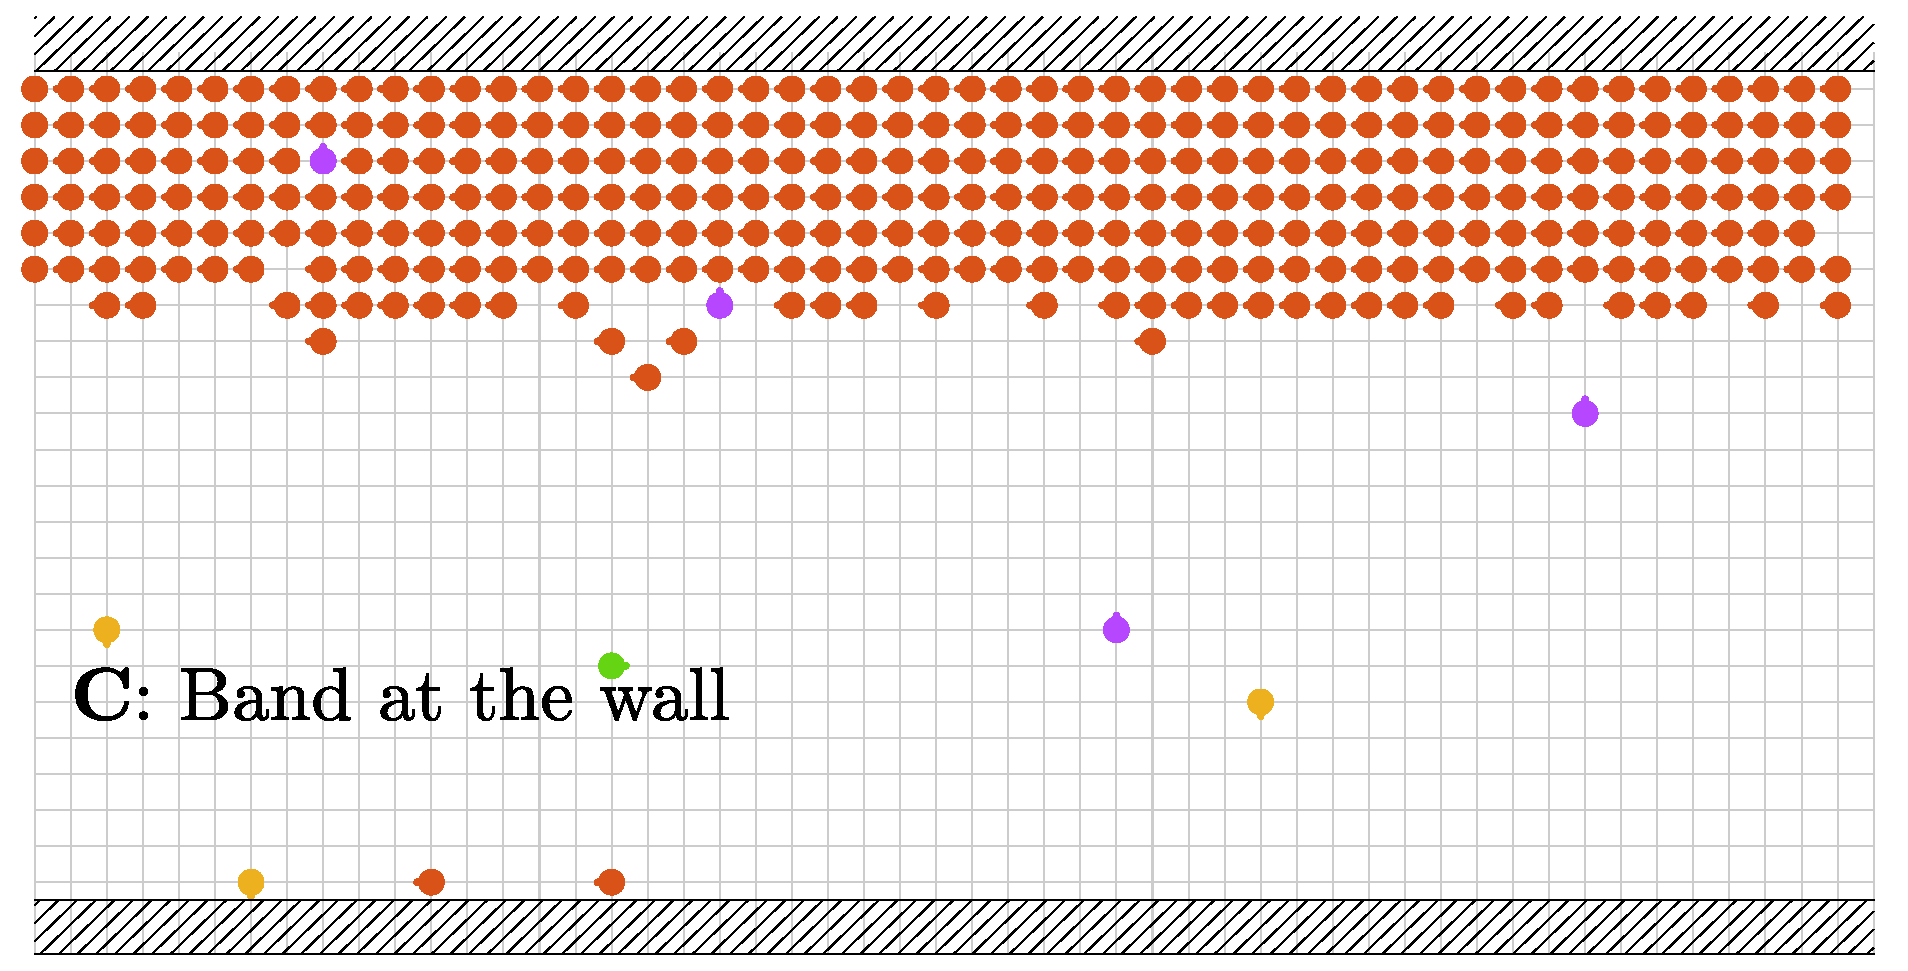
\includegraphics[width=.25\textwidth]{snap_g2.5_v1_30_t2e6}\!\!
   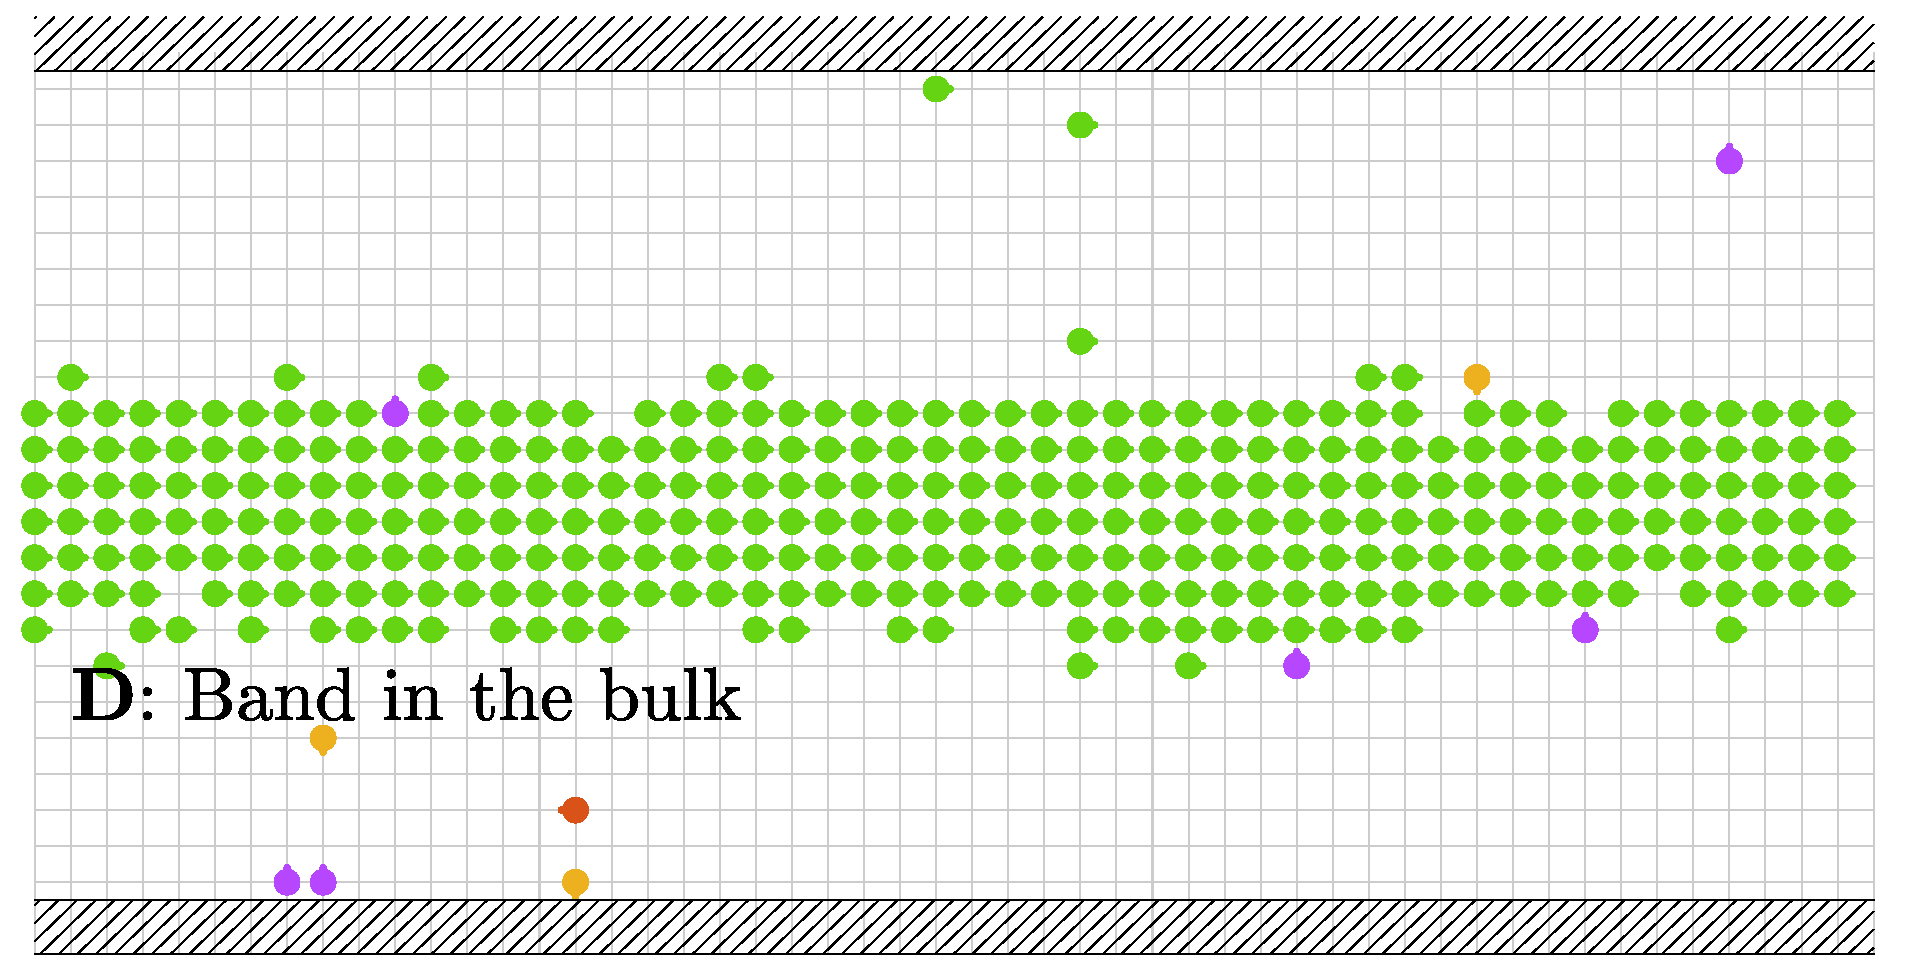
\includegraphics[width=.25\textwidth]{snap_g2.5_v1_125_t2e6}
   \caption{\label{fig:snapshots_phases} Snapshots of the lattice configuration for the four representative cases shown on the right-hand panel of Fig.~\ref{fig:param_space}.}
\end{figure*}
In the statistical steady state, the global configuration of particles can undergo dynamical transitions, where all particles change directions from left to right or migrate from one boundary to the other. One such transition is illustrated in Fig.~\ref{fig:g2_v1_15} (right panels) for $g=2$. After remaining in a band configuration along the top wall for more than $10^6$ steps, all particles abruptly migrate to reach the lower wall. During the transition, they form a structure close to a ``traffic jam'' along the bottom wall. The evolution of the order parameter and its components for this transition is shown in the top-left panel of Fig.~\ref{fig:g2_v1_15}. It is also evident that the typical transition between these macroscopic configurations can occur over very long timescales, possibly on the order of $10^6$ iterations. This should be kept in mind when estimating relevant timescales.

\subsection{Adding a mean flow towards the right}
The next set of experiments consisted in varying the parameter $v_1$ that sets the strength of the Poiseuille fluid flow within the channel. Results are summarized in Figs.~\ref{fig:param_space} and \ref{fig:snapshots_phases}. There are two main observations. First, at small $g$, the effect of a mean flow is to decrease clustering at the wall and thus to impede the formation of ``mountains'' (compare cases A and B). Second, at large values of $g$, the presence of a mean flow make the particle form bands at the center of the channel rather than near its walls (compare cases C and D).

\subsection{Notion of flux}
Our goal is to optimize the flux of active particles inside the channel, say towards the right $x>0$. However, there are several ways to define this flux. A first one could be purely kinematical. From the order parameters that we have introduced above, one can define a particle velocity profile can deduced from this order-parameter:
\begin{equation}
  \boldsymbol{V}_j(t) = U(j)\,\hat{\boldsymbol{x}} + v_0\,\boldsymbol{\Pi}_j(t).
\end{equation}
 $\Phi$ that counts the number of particles that moves to the right per unit time. We can formally define the long-term value of this flux as
\begin{equation}
\Phi_\infty = \!\!\lim_{T\to+\infty} \frac{1}{T}\left[\#\!\!\left(\!\!\begin{array}{c}\text{right motions}\\[-4pt]\text{in } [t,t+T]\end{array}\!\!\right) - \#\!\!\left(\!\!\begin{array}{c}\text{left motions}\\[-4pt]\text{in } [t,t+T]\end{array}\!\!\right)\right]\!.
\nonumber
\end{equation}
\obs{Measurements of this flux are not yet implemented in the code. One should add a counter that is updated at each horizontal migration.}

\section{A heuristic control}

We aim to maximize the flux as defined above. While our intuition is initially based on the flux obtained from the velocity profile $\boldsymbol{V}_j$, in practice, our formal goal is to optimize $\Phi\infty$. Regardless, we believe that a reasonable control strategy should be capable of (i)~disrupting clusters, especially those formed at the walls, and (ii)~increasing the likelihood of particles aligning to the right when positioned in the bulk of the channel.

As a trial to achieve these objectives, we have implemented the following process: with a specified time periodicity $\Delta t$, we apply a global action that causes all particles in the domain to change their orientation by a quarter turn, either clockwise or anticlockwise, or do nothing. The choice among these three actions depends on the discretized states of the system. Each time we apply the control, we count the number of particles $n_{\rm top}$, $n_{\rm mid}$, and $n_{\rm down}$ in the strips $h/3 < y < h$, $-h/3 < y < h/3$, and $-h < y < -h/3$, respectively, and select the region containing the largest number of particles. If it is the top region, we apply a clockwise turn only if the mean velocity in this region is oriented in the upper quadrant toward the wall. If it is the bottom region, we apply an anticlockwise turn only if the average velocity is in the lower quadrant. For the middle region, we turn clockwise or anticlockwise depending again on the orientation of the mean velocity (see Fig.~\ref{fig:sketch_heuristics}). \CC{CC: I am confused about the above description of the heuristic. Also Fig.8 is not completely clear to me.
\\
If it is the top region, we apply a clockwise turn if $\langle v_y\rangle < -|\langle vx \rangle|$ and if $v_x>0$ and an anticlokwise turn if $v_y<0$. For $\langle v_y\rangle \geq -|\langle vx \rangle|$ we don't apply the turn. See Fig.\ref{fig:Fig8_Chiara}}
\begin{figure}[t!]
    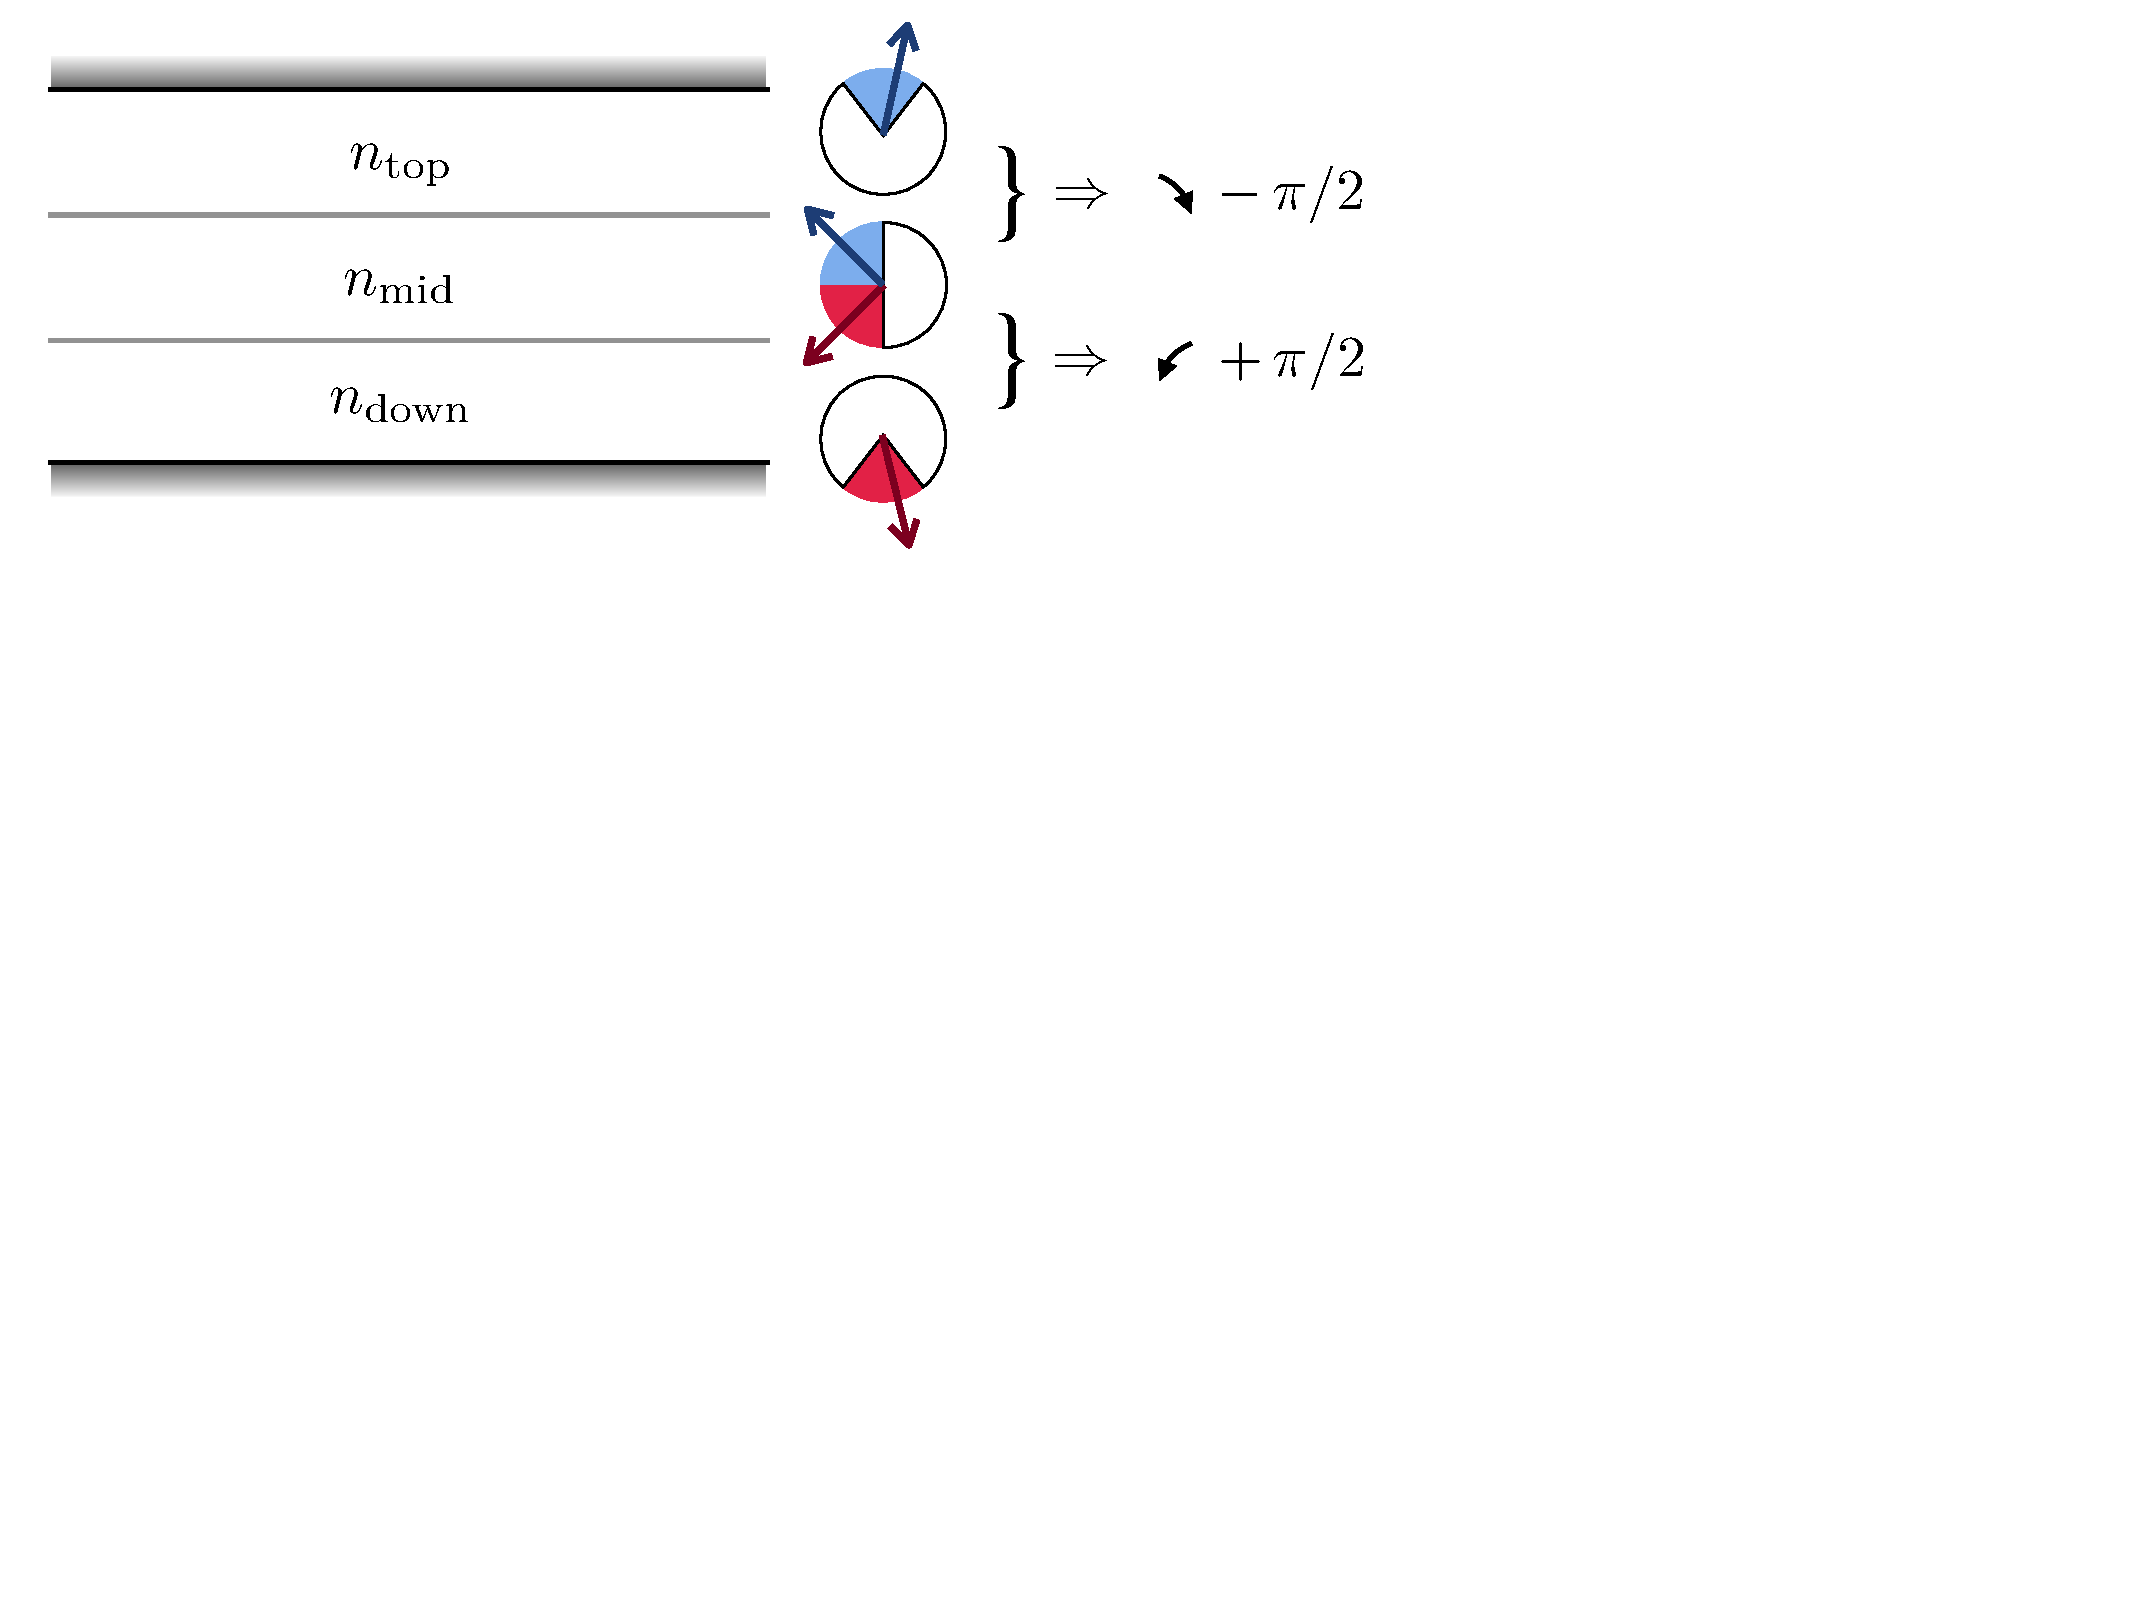
\includegraphics[width=0.8\linewidth]{sketch_heuristics}
    \caption{\label{fig:sketch_heuristics} Sketch of the heuristic policy.}
\end{figure}

\begin{figure}[t!]
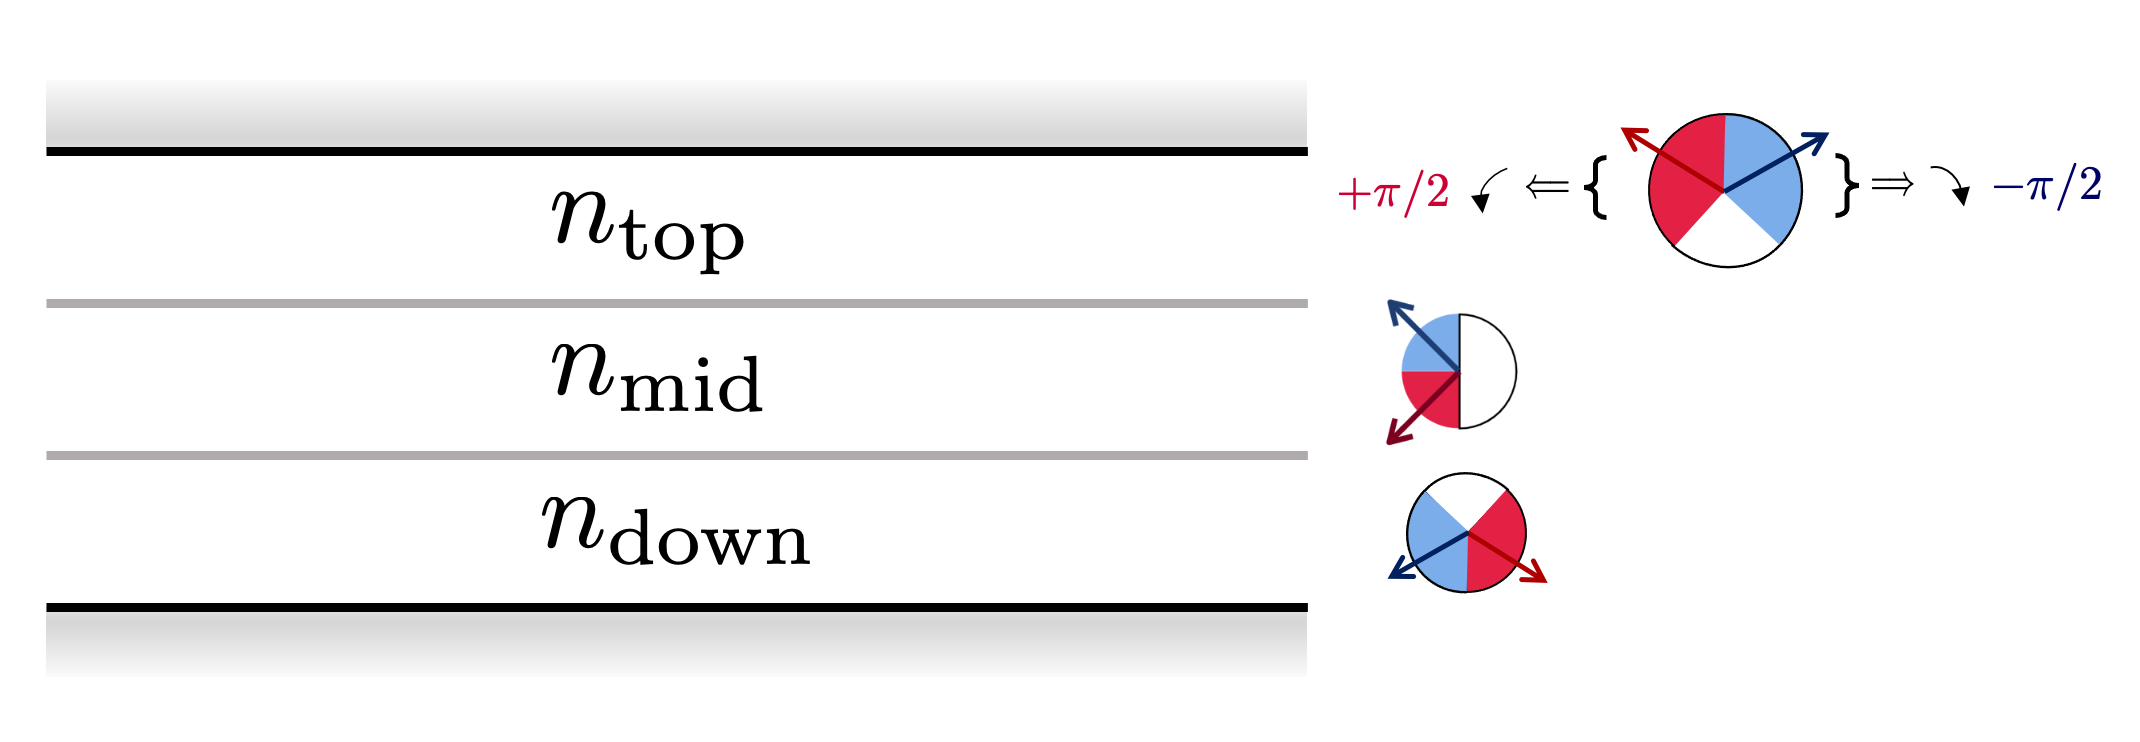
\includegraphics[width=01\linewidth]{figs/Fig8_Chiara.png}
    \caption{ \CC{CC: This should be what the heuristic strategies are doing in the code. Am I wrong? Blue: clockwise rotation, red: anticlockwise turn, white: do nothing.}\label{fig:Fig8_Chiara}}
\end{figure}

Preliminary results with this control show that it is able to disrupt the clusters, at least at small values of $g$ (see Fig.~\ref{fig:swarm_channel}). \obs{Further analysis, and in particular a quantification of fluxes, is required.}
\begin{figure}[H]
    \centering
    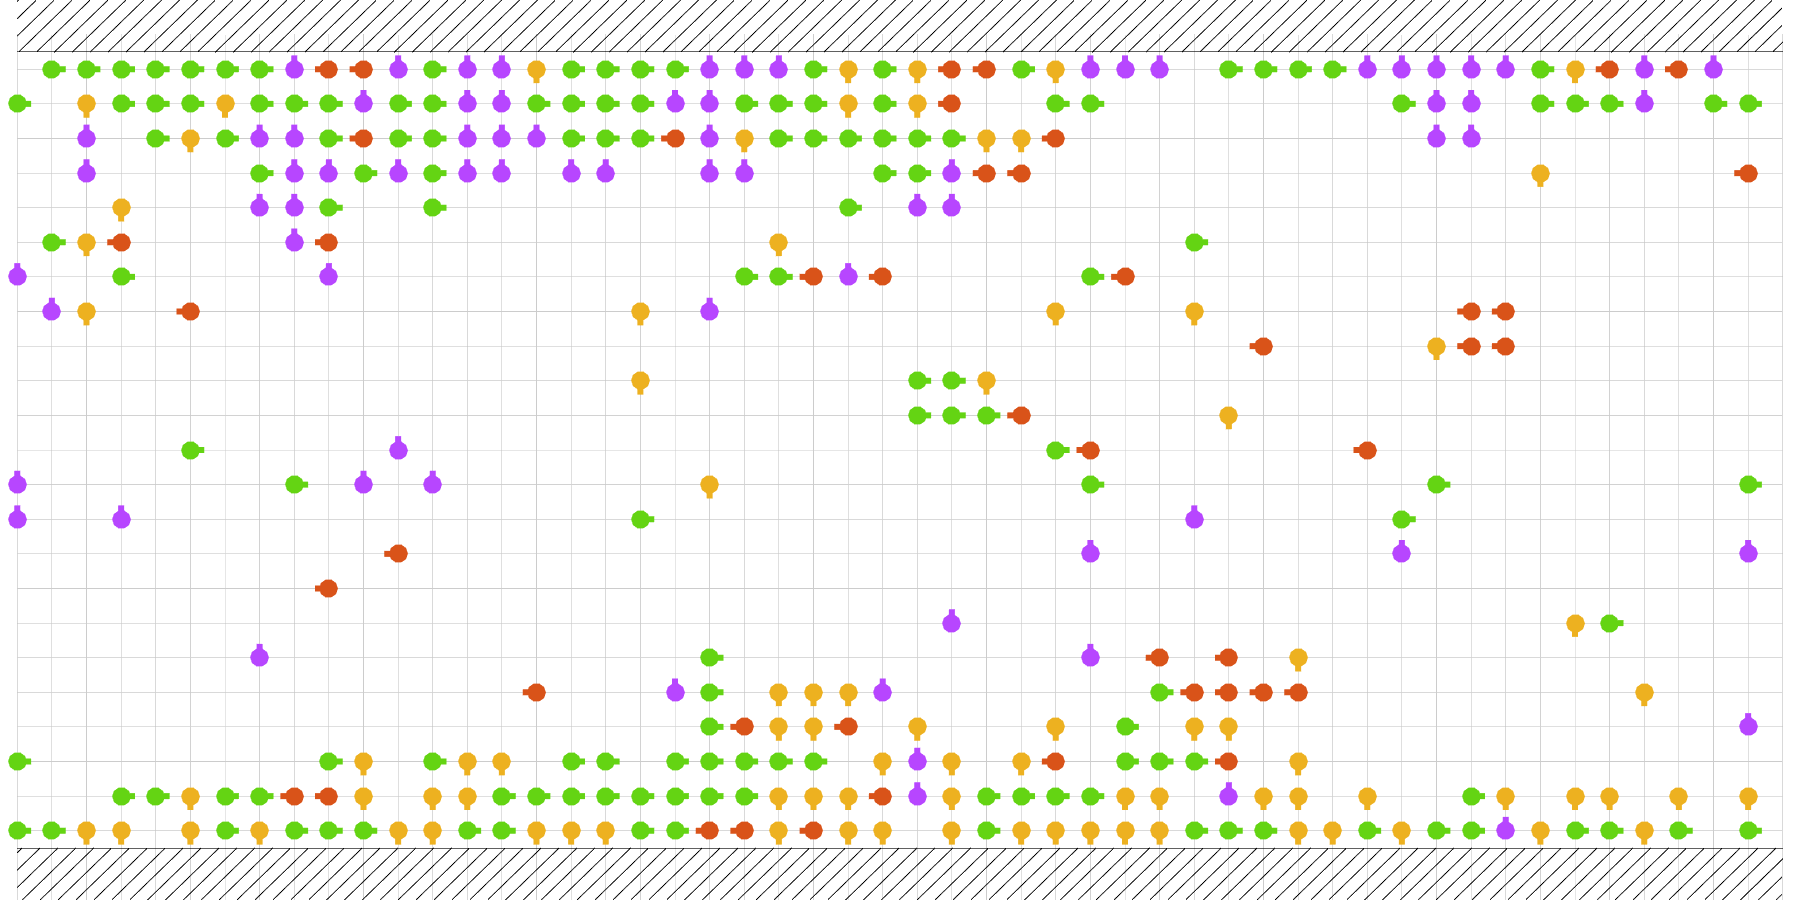
\includegraphics[width=0.62\linewidth]{swarm_channel_nocontrol}\\[4pt]
    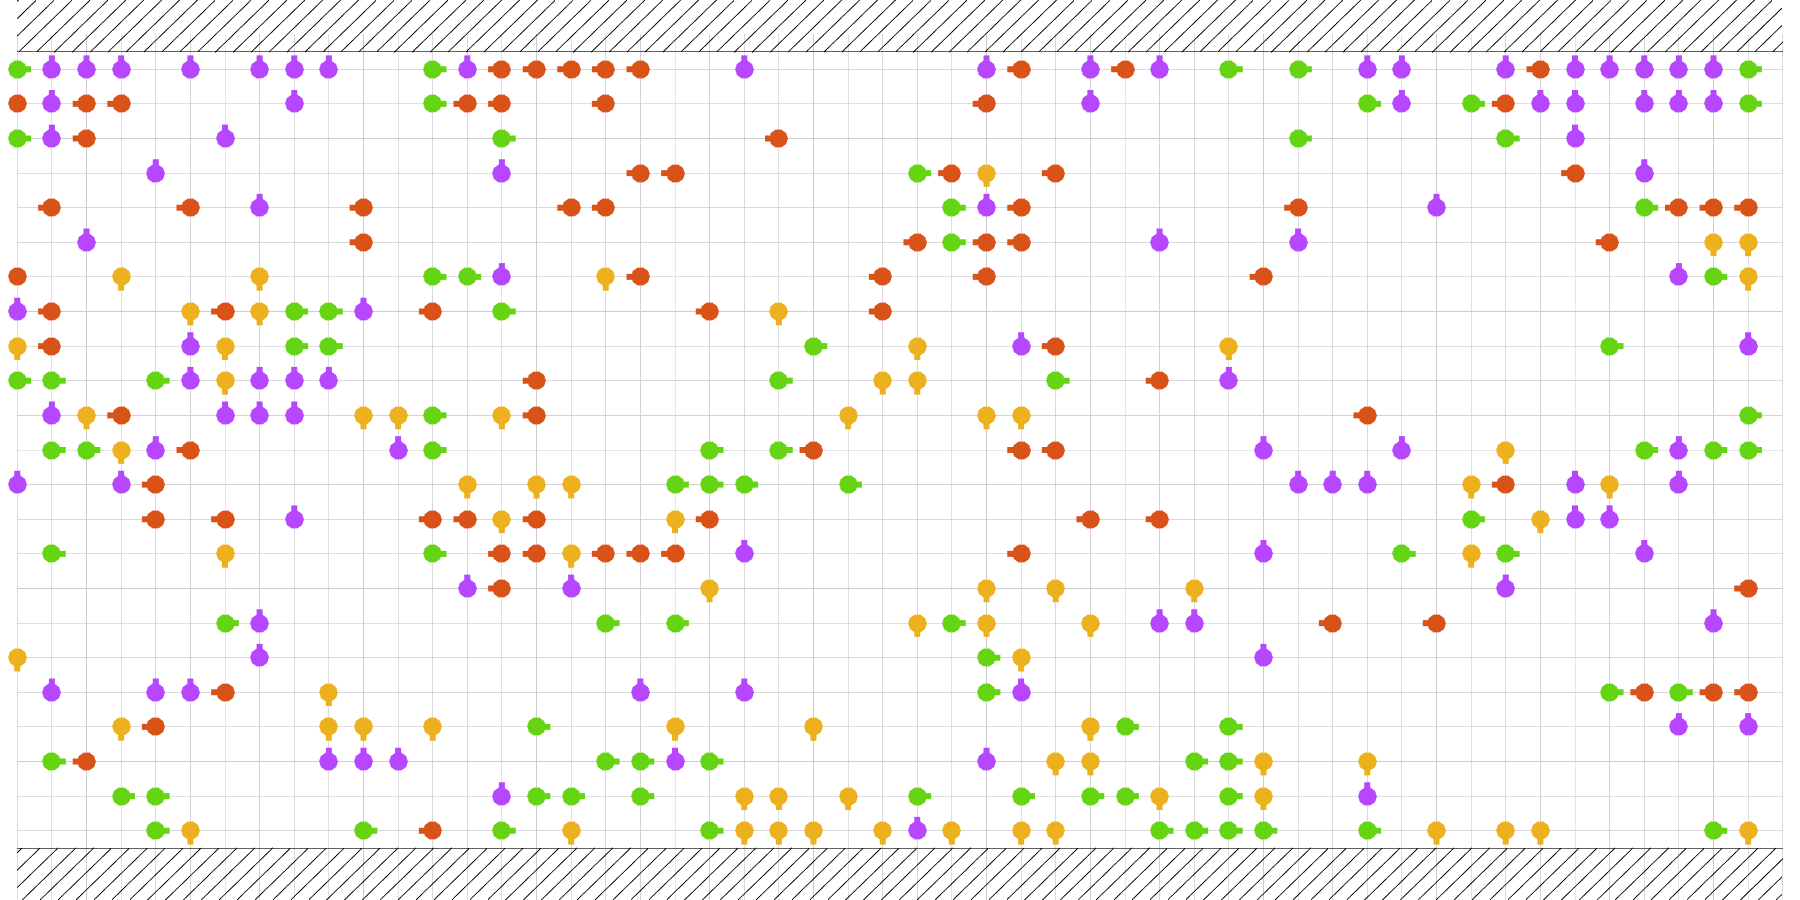
\includegraphics[width=0.62\linewidth]{swarm_channel_control}
    \caption{\label{fig:swarm_channel} Lattice configurations without applying (top) and when applying (bottom) the heuristic policy for $g=1$ and $v_1=50$.}
\end{figure}

\section{Todos}
\noindent\obs{\textbf{In the code of the model}}\\
\obs{$\bullet$ Implement the restarts}\\
\obs{$\bullet$ Add measurement of the fluxes}\\
\obs{$\bullet$ Recompute the rates only locally and not globally at each steps}\\
\obs{$\bullet$ Write lattice output in a more frugal (binary) manner}

\

\noindent\obs{\textbf{Simulations}}\\
\obs{$\bullet$ Longer runs for more statistics with the current resolution}\\
\obs{$\bullet$ Higher resolutions for fixed parameters $g$ and $v_1$}\\
\obs{$\bullet$ Vary the aspect ratio (box length), keeping resolution fixed}

\

\noindent\obs{\textbf{Learning}}\\
\obs{$\bullet$ Implement the gymnasium wrappers}\\
\obs{$\bullet$ Test usual $Q$ learning with simple discretised states}\\
\obs{$\bullet$ Test deep $Q$-learning with the whole lattice as an input of the network}

\

\begin{acknowledgments}
\end{acknowledgments}

\bibliography{references}
\end{document}
